\documentclass[10pt]{article}
\usepackage[preprint]{tmlr}
\usepackage{fontspec}
\setmainfont{cmunrm.ttf}[Path=fonts/,BoldFont=cmunbx.ttf,ItalicFont=cmunti.ttf,BoldItalicFont=cmunbi.ttf]
\setsansfont{cmunss.ttf}[Path=fonts/,BoldFont=cmunsx.ttf,ItalicFont=cmunsi.ttf,BoldItalicFont=cmunso.ttf]
\setmonofont{DejaVu Sans Mono}[Scale=0.82]
\usepackage[russian,english]{babel}
\babelprovide[import,main]{russian}
\usepackage{amsmath,amssymb,graphicx,booktabs,tabularx,longtable,array,tikz,flafter,needspace}
\usepackage[unicode,colorlinks=true,linkcolor=blue!45!black,urlcolor=blue!45!black,citecolor=blue!45!black]{hyperref}
\usetikzlibrary{arrows.meta}
\definecolor{concept}{HTML}{7570B3}
\definecolor{soft}{HTML}{8C8C8C}
\newcolumntype{Y}{>{\raggedright\arraybackslash}X}
\newcommand{\ci}[2]{[#1;\,#2]}
\title{Оценка обучения на понятиях\\с помощью контрольных меток}
\author{Рабочая русскоязычная версия}
\begin{document}
\selectlanguage{russian}
\maketitle
\begin{abstract}
Модели на понятиях обучают решать основную задачу и предсказывать заданные человеком признаки объектов. Чтобы оценить, чему ещё научилась модель, проверяют, можно ли по её внутренним векторам предсказывать другие признаки, метки которых не использовали при обучении. Качество такого предсказания далее называем читаемостью признаков. Однако высокая читаемость сама по себе не показывает, какую роль в её достижении сыграли метки обучающих понятий. Мы исследуем роль этих меток с помощью контрольных замен: например, вместо ответов о признаках птиц используем случайный код, закреплённый за каждым видом. В перепроверке моделей Concept Embedding Models на CUB, где метки заданы на уровне вида и проверка проходит на фотографиях уже известных видов, точность предсказания других признаков остаётся высокой и после такой замены. Структурированный поиск в выбранном корпусе показывает, что сравнения с заменой обучающих меток встречаются редко. На втором примере, поиске подпонятий в HiCEM, показываем, что оценка самого поиска и оценка последующего предсказания найденных признаков могут приводить к разным выводам о роли обучающих меток. Эти результаты показывают, зачем отделять успешное предсказание новых признаков от объяснения его причин. Мы рассматриваем, какие свойства контрольных меток необходимо учитывать при сравнении и как выбор оценки меняет вывод о пользе обучения на понятиях.
\end{abstract}

\section{Введение}
При обучении модели машинного обучения можно использовать разметку не только для основной задачи, но и для предсказания отдельных свойств объектов. В моделях на понятиях такие свойства называют \emph{понятиями}, а их предсказания используют для решения основной задачи \citep{cbm,cem}. Например, при распознавании изображений птиц основной задачей может быть определение вида, а понятиями --- признаки внешности: белое горло, изогнутый клюв, полосы на крыльях. Ответы «да» или «нет» о наличии каждого признака служат \emph{метками понятий}. Но чему ещё учится модель, когда ей сообщают такую разметку?

Для анализа обученных сетей используют \emph{пробы}: по внутренним представлениям сети обучают отдельную модель предсказывать интересующее свойство. Такой подход применяется к визуальным и языковым представлениям \citep{alain,conneau}. В частности, можно проверять свойства, метки которых не использовали при обучении самой сети: так оценивают новые признаки в моделях на понятиях \citep{cem} и свойства социальных сцен после обучения на человеческих оценках сходства видео \citep{garcia}.

Поясним устройство пробы на примере птиц. Обрабатывая фотографию, сеть вычисляет внутренний вектор чисел --- её представление этой фотографии. После обучения веса сети фиксируют. Затем по её векторам обучают отдельную модель предсказывать признак, метки которого не использовали при обучении сети: например, цвет горла, если дополнительная разметка описывала только клюв и крылья. Если отдельная модель линейная, её называют \emph{линейной пробой}. В опыте с птицами её точность на фотографиях, не использованных для обучения пробы, будем называть \emph{читаемостью признака}. Геометрический смысл этой проверки показан на рисунке~\ref{fig:readability}.

\begin{figure}[htbp]
\centering
\begin{tikzpicture}[x=1cm,y=1cm,font=\small]
\foreach \shift/\title in {0/{Ответы трудно разделить},8/{Ответы легко разделить}} {
\begin{scope}[xshift=\shift cm]
\filldraw[fill=black!2,draw=black!18,rounded corners=3pt] (0,0) rectangle (7,3.8);
\node at (3.5,3.45) {\title};
\draw[-{Stealth},soft] (.6,.55)--(6.5,.55);
\draw[-{Stealth},soft] (.6,.55)--(.6,3.0);
\draw[concept,dashed,thick] (3.6,.7)--(3.6,2.95);
\end{scope}}
\foreach \x/\y in {1.3/1.2,2/2.6,2.7/1.6,4.2/2.4,5.4/1.3,5.9/2.7}
 \fill[concept] (\x,\y) circle (3pt);
\foreach \x/\y in {1.4/2.3,2.3/1,3/2.7,4.5/1,5/2,6.1/1.7}
 \draw[soft,fill=white,thick] (\x,\y) circle (3pt);
\foreach \x/\y in {9.3/1.2,9.4/2.3,10/2.6,10.3/1,10.7/1.6,11/2.7}
 \fill[concept] (\x,\y) circle (3pt);
\foreach \x/\y in {12.2/2.4,12.5/1,13/2,13.4/1.3,13.9/2.7,14.1/1.7}
 \draw[soft,fill=white,thick] (\x,\y) circle (3pt);
\fill[concept] (3.1,-.4) circle (3pt);
\node[anchor=west] at (3.3,-.4) {признак есть};
\draw[soft,fill=white,thick] (7,-.4) circle (3pt);
\node[anchor=west] at (7.2,-.4) {признака нет};
\end{tikzpicture}
\caption{Читаемость признака: условная двумерная схема. Точка --- представление одной фотографии; цвет --- ответ о проверяемом признаке. Линейная проба учится проводить разделяющую границу и проверяется на других фотографиях. Справа такая граница хорошо разделяет ответы. Схема показывает, что измеряет проба; она не объясняет причину разделимости и не изображает результаты экспериментов.}
\label{fig:readability}
\end{figure}

Высокая читаемость означает, что по внутреннему вектору можно предсказать проверяемый признак. Однако откуда взялась эта возможность? Сеть видела фотографии, училась определять виды и могла быть предварительно обучена на других фотографиях. Поэтому цвет горла может хорошо предсказываться и без дополнительной задачи предсказания признаков клюва и крыльев. Высокая читаемость сама по себе не показывает, какую роль в её достижении сыграли метки обучающих понятий.

Мы исследуем это различие, меняя дополнительные метки при обучении сети. Например, вместо ответов о внешности каждому виду птиц назначаем случайный двоичный код, одинаковый для всех его фотографий. Сеть учится определять вид и предсказывать этот код. Затем обучаем линейные пробы предсказывать по её векторам те же настоящие признаки, которые не использовали при обучении сети. Метки, которыми мы заменяем настоящие ответы для такого сравнения, будем называть \emph{контрольными}. Набор признаков, метки которых используются при обучении сети, далее обозначаем $A$, а набор признаков для последующей оценки --- $B$. Метки $B$ используются при обучении проб, но не самой сети.

\paragraph{Основные вклады работы.}
Работа вносит четыре вклада:
\begin{itemize}
\item разделяет два вопроса, которые часто объединяют: можно ли предсказать признак по представлению модели и связано ли это с содержанием меток, использованных при обучении;
\item перепроверяет эксперимент CEM с несколькими контрольными заменами и показывает, что высокая читаемость новых признаков сохраняется при случайном коде, а вывод о преимуществе настоящих меток зависит от выбранного контроля;
\item проводит структурированный обзор выбранного корпуса работ и фиксирует, как часто в нём встречаются сравнения с заменой обучающего сигнала, вместе с протоколом отбора и ограничениями такого подсчёта;
\item рассматривает второй случай, Concept Splitting в HiCEM, где отдельно сравниваются качество предсказания найденных подпонятий и число найденных соответствий, и показывает, какие свойства контрольных меток и какие показатели оценки необходимо учитывать при подобных сравнениях.
\end{itemize}

Сначала повторяем эксперимент авторов Concept Embedding Models (CEM) и добавляем сравнение с контрольными метками (раздел~\ref{sec:cem}). В нём высокая читаемость $B$ получается и при обучении на случайном коде вида. Затем рассматриваем, как часто в литературе проверяют результат заменой обучающих меток (раздел~\ref{sec:prevalence}). Наконец, переходим к методу Concept Splitting из работы о HiCEM \citep{hicem}, который ищет более подробные признаки в представлениях модели, обученной предсказывать общие признаки (раздел~\ref{sec:hicem}). В этом случае оказывается важно учитывать не только качество, но и число найденных признаков. В разделе~\ref{sec:discussion} «Обсуждение» сопоставляем результаты двух перепроверок, обсуждаем дополнительные опыты и ограничения и формулируем, как выбирать контроль и показатель под конкретный вопрос. В разделе~\ref{sec:conclusion} суммируем основные выводы.

\section{Перепроверка CEM}\label{sec:cem}
\subsection{Какое утверждение проверяем}
В §5.3 статьи о CEM авторы интерпретируют более высокую точность CEM по сравнению с Hybrid-CBM при предсказании понятий, не использованных при обучении, как свидетельство переносимости информации о понятиях и связывают такую переносимость с большей интерпретируемостью представлений CEM. Для проверки этого наблюдения по представлениям предсказывают признаки, метки которых не использовали при обучении сети \citep[§5.3, приложение~A.9]{cem}. Эксперимент проводится на фотографиях птиц. CEM сравнивают с Hybrid-CBM --- другой архитектурой, обученной определять те же виды и признаки. Рассуждение имеет четыре звена:
\begin{enumerate}
\item сеть обучают определять вид и предсказывать признаки $A$;
\item по её представлению обучают линейные пробы для остальных признаков $B$;
\item у CEM точность проб оказывается выше, чем у Hybrid-CBM, обученной на тех же $A$;
\item авторы связывают более высокую точность при предсказании понятий, не использованных при обучении, с переносимостью информации о понятиях и большей интерпретируемостью представлений CEM.
\end{enumerate}
Мы сначала воспроизводим сравнение архитектур из третьего звена. Затем проверяем, нужна ли CEM настоящая разметка $A$, чтобы получить высокую читаемость и превысить результат Hybrid-CBM. Для этого обучаем CEM на контрольных метках. Если пробы хорошо предсказывают $B$ и после замены меток $A$, это показывает, что высокая точность достижима без настоящей разметки $A$. Так мы оцениваем, насколько наблюдение авторов поддерживает вывод о роли содержания обучающих меток; интерпретируемость как общее свойство представления напрямую не измеряем. Сам результат о возможности предсказывать $B$ по векторам CEM при этом не опровергается. Дополнительное сравнение проверяет, можно ли получить такой результат и при обучении на других метках.

\subsection{Постановка авторов и наше повторение}
Чтобы повторить сравнение, сначала рассмотрим, на каких данных авторы обучали модели, чем отличаются их внутренние векторы и как по этим векторам предсказывают $B$.

Авторы проводят этот эксперимент на CUB-200-2011 --- наборе фотографий птиц 200 видов \citep{cub}. Мы используем тот же набор и подготовку разметки из работы CEM: 112 признаков с ответами «да» или «нет» \citep[приложения~A.3.4 и A.9]{cem}. Разметка задаётся для вида целиком: все фотографии одного вида получают одинаковые ответы, даже если признак не виден на отдельном снимке. Следуя схеме авторов, в каждом из пяти повторов используем 28 признаков как $A$, остальные 84 --- как $B$ (рисунок~\ref{fig:data}). Между повторами меняются набор $A$ и начальные веса сети. При проверке используются другие фотографии уже известных модели видов.

\begin{figure}[htbp]
\centering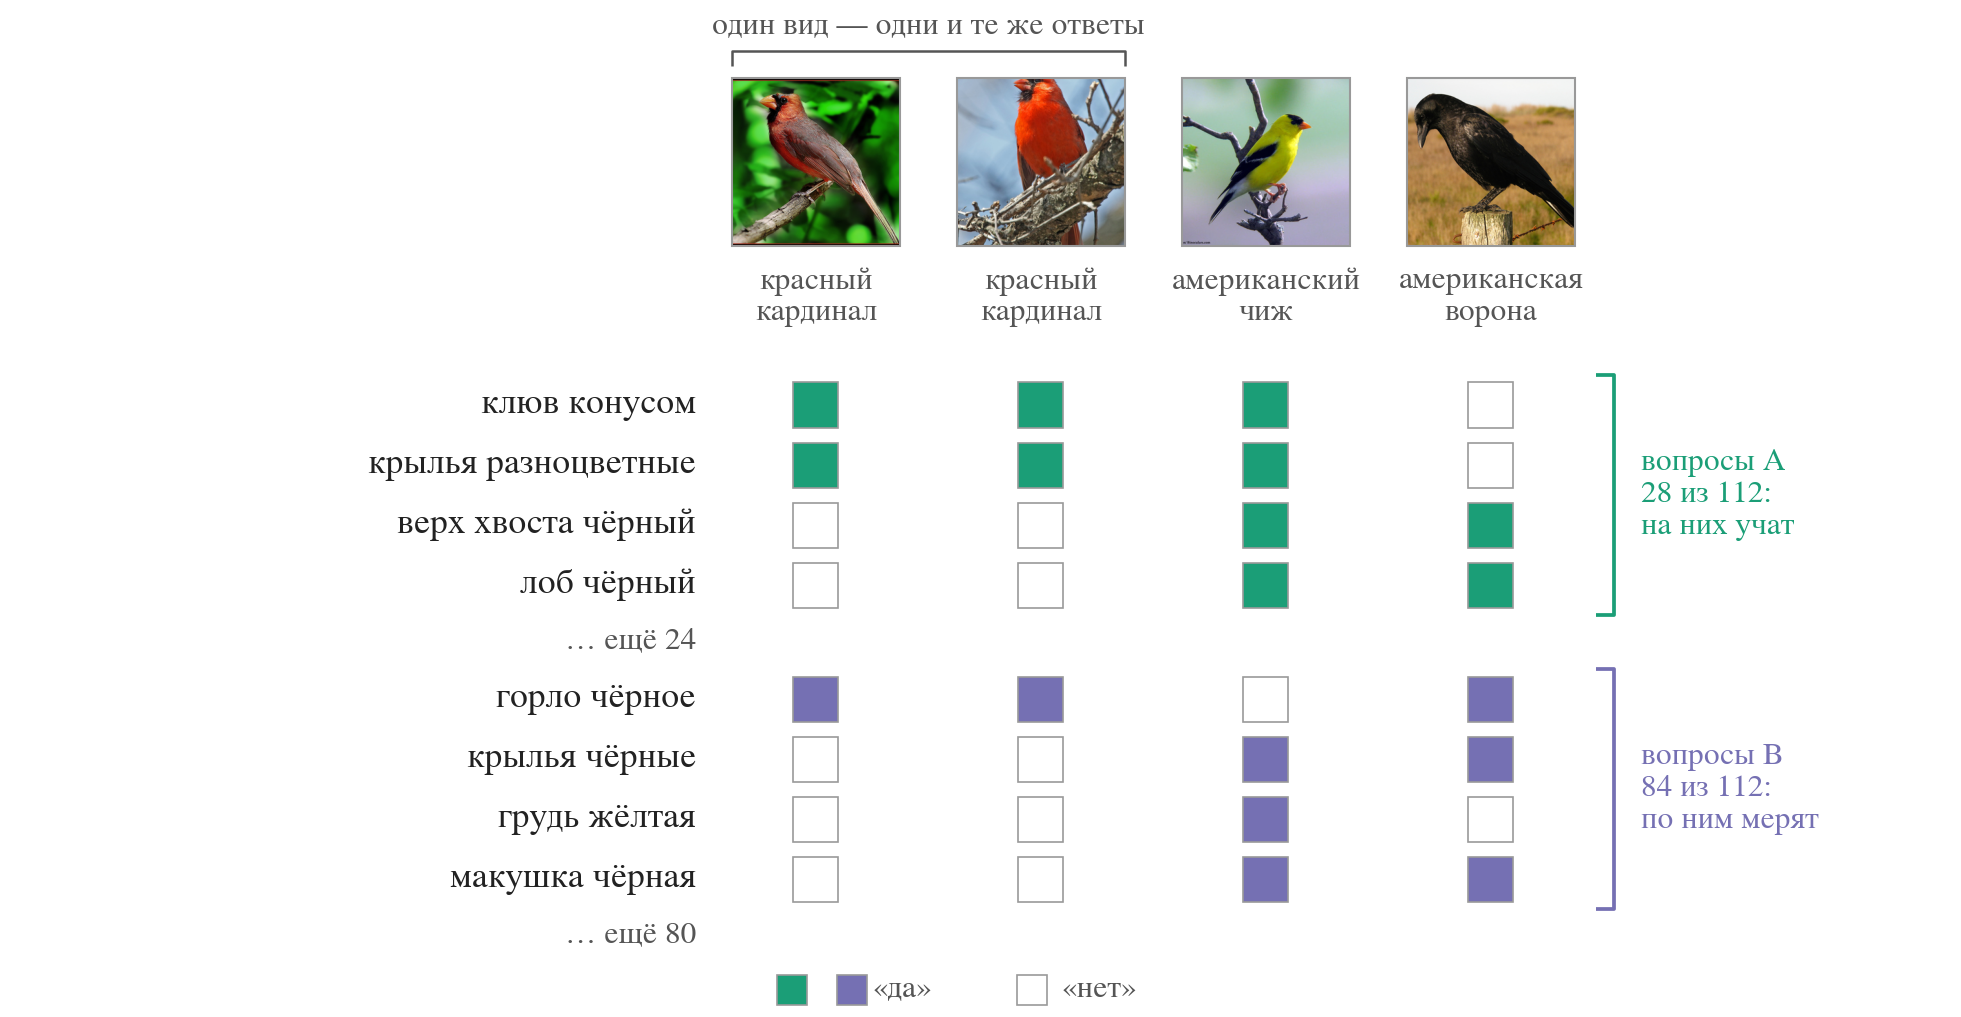
\includegraphics[width=\linewidth]{../figures/v2_data.png}
\caption{Примеры фотографий и меток, заданных на уровне вида в CUB. Показана часть признаков одного повтора. Метки $A$ используются при обучении сети, $B$ --- позднее, для обучения и проверки линейных проб.}
\label{fig:data}
\end{figure}

Для обеих архитектур авторы используют предварительно обученную ResNet-34, которая преобразует фотографию в вектор визуальных признаков \citep[приложение~A.6]{cem}. Эту основу мы сохраняем в повторении. Из полученных визуальных признаков каждая модель строит вектор $z$ из 448 чисел, по которому определяют вид птицы. CEM вычисляет для каждого обучающего понятия $i$ вектор $z_i$ из 16 чисел. Вектор $z_i$ представляет собой взвешенную сумму двух вычисляемых сетью векторов: один соответствует наличию понятия, другой --- его отсутствию. Веса этой суммы --- предсказанная вероятность наличия понятия и её дополнение до единицы. В процедуре авторов при обучении часть предсказанных вероятностей заменяют настоящими метками понятий; в наших контрольных опытах для этой подстановки используются контрольные метки. При оценке обученной сети метки ей уже не подставляют. Объединение 28 векторов даёт $z$. Hybrid-CBM вместо этого объединяет 28 вероятностей понятий и 420 дополнительных чисел, которые сеть учится вычислять для определения вида. Итоговая размерность одинакова, но устройство представления различается (рисунок~\ref{fig:models}).

\begin{figure}[htbp]
\centering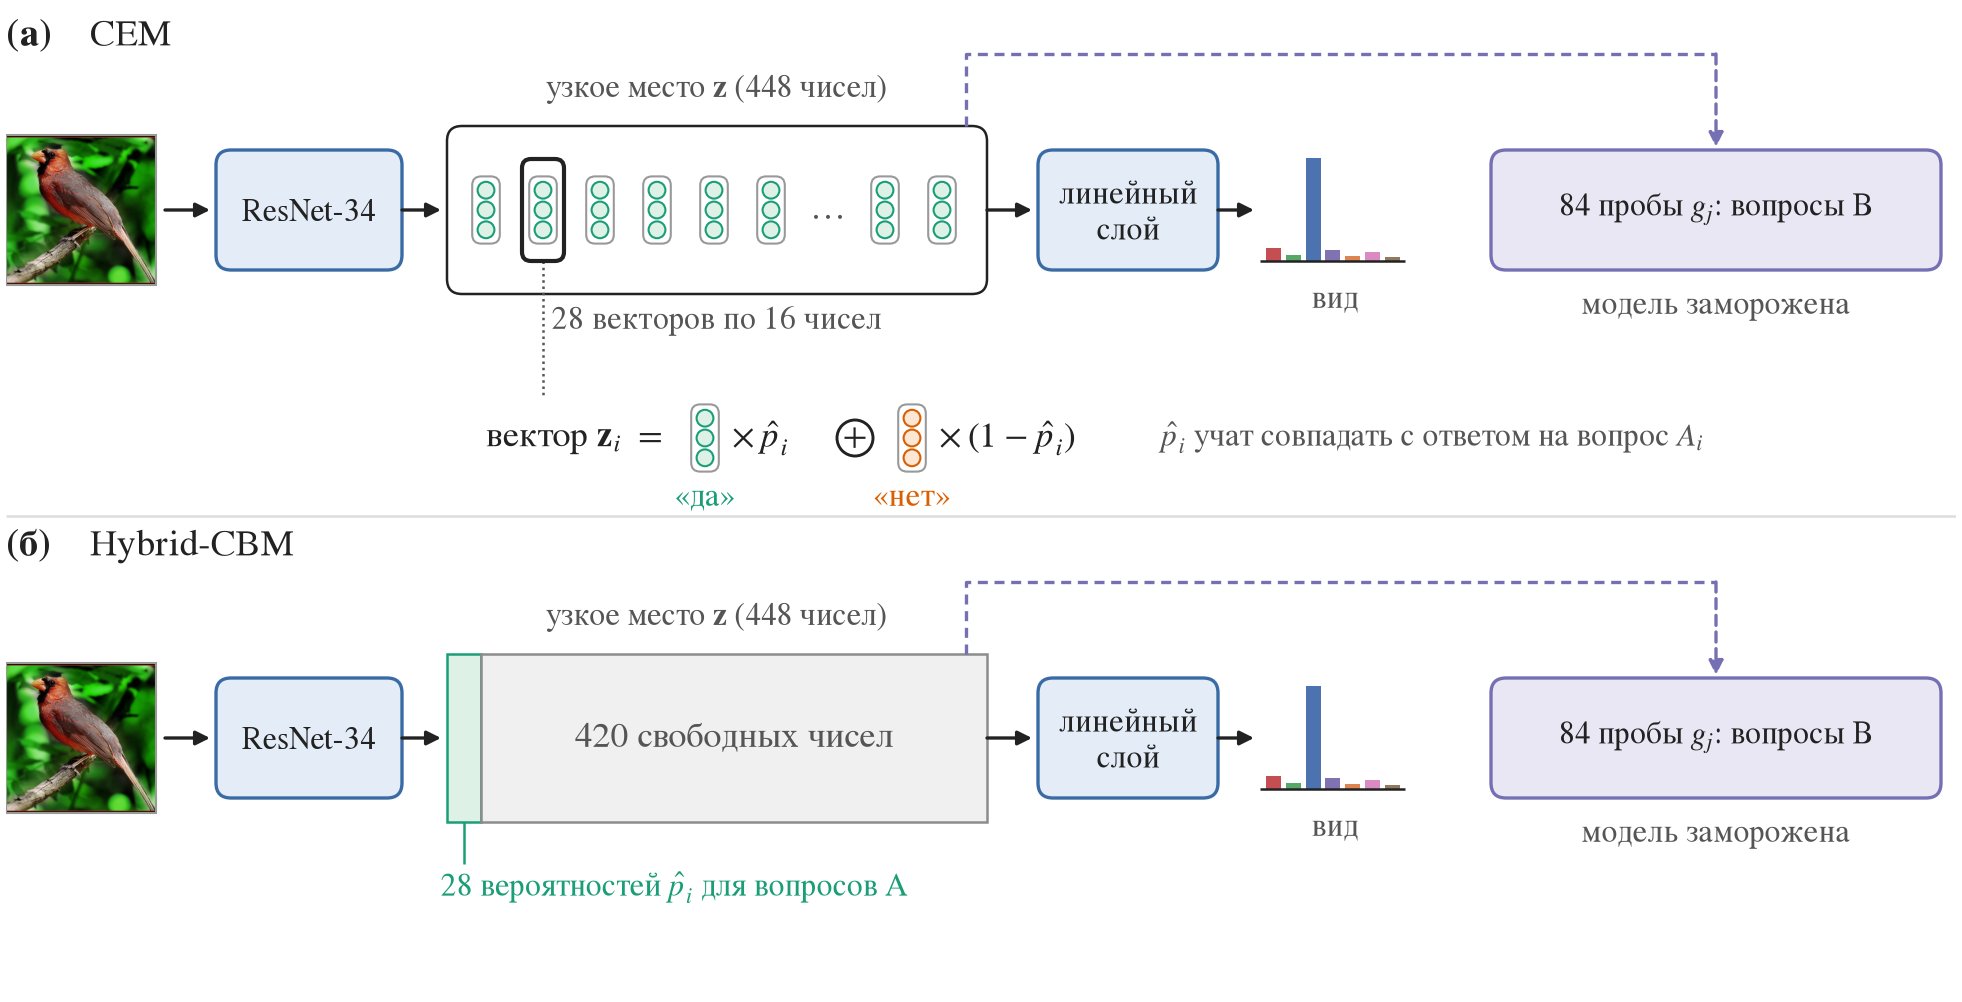
\includegraphics[width=\linewidth]{../figures/v2_models.png}
\caption{Устройство сравниваемых представлений и последующая оценка. Hybrid-CBM на настоящих $A$ служит общим ориентиром: с ней сравниваем CEM как на настоящих, так и на контрольных метках. Сеть сначала обучают и замораживают; только после этого по её векторам обучают пробы на $B$.}
\label{fig:models}
\end{figure}

Авторы оценивают представления с помощью отдельных логистических регрессий для 84 признаков $B$ \citep[приложение~A.9]{cem}. Мы повторяем эту схему: для каждого признака обучаем линейную пробу с ответом «да» или «нет». Её входом служит вектор $z$ обученной сети. Пробе показывают настоящие ответы $B$ для учебных фотографий, а точность оценивают на проверочных. Сама сеть на этом этапе не меняется. Среднюю точность 84 проб называем \emph{читаемостью $B$}. Ответ «нет» встречается часто: средняя по 84 признакам точность постоянного ответа «нет» составляет около 81.8\%. Поэтому высокую точность нужно рассматривать вместе со сравнением условий обучения. Авторская реализация проб недоступна, поэтому пробы реализованы нами; их настройки и расчёт интервалов приведены в приложении~\ref{app:cem}.

\subsection{Повторение сравнения архитектур}
В исходной статье сообщается читаемость 94.33\% для CEM и 91.83\% для Hybrid-CBM. В нашем повторении --- 95.12\% и 94.76\%. Разность составляет $+0.36$ процентного пункта с 95\%-м доверительным интервалом $\ci{-0.18}{+0.90}$ по пяти парным повторам. Интервал включает и отрицательные, и положительные значения, поэтому по этим повторам нельзя установить преимущество CEM по точности.

Размерность Hybrid-CBM в тексте и коде статьи различается. Здесь мы используем вариант из описания статьи: его итоговая размерность совпадает с размерностью CEM. Для варианта Hybrid-CBM из кода преимущество CEM по точности установлено (приложение~\ref{app:cem}). Для выбранного здесь варианта при других настройках пробы доверительный интервал разности точностей также включает ноль; по другой оценке качества, учитывающей ранжирование положительных ответов (average precision, AP), CEM имеет преимущество. Эти дополнительные результаты приведены в приложении~\ref{app:cem}. Далее проверяем, как замена меток при обучении CEM меняет точность проб и её разность с результатом Hybrid-CBM на настоящих метках.

\subsection{Высокая читаемость при обучении на случайном коде}
Даже если преимущество одной архитектуры над другой невелико, остаётся основной вопрос: нужна ли настоящая разметка $A$ для полученной высокой точности? Назначим каждому виду случайный код из 28 нулей и единиц. Все фотографии одного вида получают один и тот же код; коды разных видов различны. При назначении кода настоящие $A$, $B$ и изображения не используются. Сеть по-прежнему учится определять вид, но вместо ответов о внешности предсказывает случайный код своего вида.

Архитектуру и процедуру обучения сохраняем. В частности, сохраняем коэффициенты, определяющие вес ошибок в дополнительных ответах: они такие же, как при обучении на настоящих $A$. Иначе замена меток одновременно изменила бы и эти настройки. Результаты приведены в таблице~\ref{tab:cem}.

\begin{table}[htbp]
\centering
\caption{Читаемость $B$: средняя точность пяти повторов. В последней строке веса ошибок такие же, как при настоящих $A$.}
\label{tab:cem}
\begin{tabularx}{\linewidth}{Yr}\toprule
Обучение & Точность, \% \\\midrule
CEM: только определение вида & 92.72\\
Hybrid-CBM: вид и настоящие $A$ & 94.76\\
CEM: вид и настоящие $A$ & 95.12\\
CEM: вид и случайный код & 95.39\\\bottomrule
\end{tabularx}
\end{table}

После обучения CEM на случайном коде точность проб для $B$ остаётся высокой: 95.39\% против 95.12\% на настоящих $A$. Разность «случайный код минус настоящие $A$» равна $+0.27$ пункта, интервал $\ci{-0.27}{+0.80}$. Он недостаточно узок, чтобы считать условия эквивалентными по принятому критерию (приложение~\ref{app:cem}). При этом в выполненных запусках высокую точность можно получить и без настоящей дополнительной разметки.

Теперь вернёмся к третьему звену --- сравнению с Hybrid-CBM на настоящих $A$. CEM на случайном коде превосходит этот результат на $+0.63$ пункта, интервал $\ci{+0.04}{+1.22}$. Здесь Hybrid-CBM служит одним и тем же ориентиром: её не переобучали на случайных метках. Таким образом, превышение её точности возможно без обучения CEM на настоящих метках $A$. Этот опыт не сравнивает две архитектуры, обе обученные на случайном коде.

Почему такая читаемость возможна? В этих данных и случайный код, и ответы $B$ постоянны внутри вида. Информация о виде поэтому может помогать линейной пробе отвечать на вопросы $B$. Это правдоподобное объяснение того, почему отсутствие настоящих $A$ совместимо с высокой читаемостью; проведённый опыт не устанавливает конкретный механизм изменения представления.

CEM, обученная только определять виды, также даёт высокую читаемость --- 92.72\%. В этом варианте сеть обучается, но ошибки в ответах о понятиях не влияют на обновление её весов, а предсказания понятий не подменяются метками. В этой модели признаки $B$ хорошо предсказываются и без дополнительного обучения на метках понятий. Этот опыт не разделяет вклад предварительного обучения и последующего обучения определению вида.

\subsection{Что меняется при другом контроле}
Случайный код показывает, что высокая читаемость возможна без настоящих ответов $A$. Однако это сравнение не позволяет отделить роль содержания меток от других различий между условиями. Случайный код различает все 200 видов, тогда как настоящие метки $A$ у некоторых видов совпадают: в наших повторах они задают 153--185 различных наборов ответов. Кроме того, при замене могут измениться доля единиц и связи между ответами. Поэтому разность между настоящими $A$ и случайным кодом нельзя интерпретировать как оценку вклада смысла меток.

Далее мы проверяем устойчивость этого наблюдения к выбору контроля. Три следующие замены сохраняют разные свойства настоящих меток и нарушают другие; их результаты помогают понять, от каких свойств зависит сравнение, но ни одна из этих разностей не является оценкой чистого смыслового вклада. В контроле «чужой вид» случайно переставляем целые наборы $A$ между видами, так что каждому виду достаётся набор другого. Частоты отдельных ответов и их совместные комбинации сохраняются. «Перетасовка» независимо перемешивает метки каждого признака между видами: частоты остаются прежними, а комбинации меняются. Для контроля «по внешности» усредняем визуальные векторы предварительно обученной ResNet-34 по фотографиям каждого вида и разделяем их случайными гиперплоскостями. Метка определяется тем, по какую сторону границы находится вектор вида. Построение сохраняет частоты положительных меток на уровне видов и приближённо воспроизводит их попарные корреляции. Такие метки зависят от визуальных представлений и могут сохранять связь с $B$. Подробные свойства этих замен приведены в приложении~\ref{app:cem}.

\begin{table}[htbp]
\centering\small
\caption{Чувствительность результата к контрольным меткам. Положительная разность означает преимущество настоящих $A$. Показаны 95\%-е доверительные интервалы средних разностей по парным повторам. Поправка на множественные сравнения не применялась.}
\label{tab:controls}
\begin{tabularx}{\linewidth}{Yrr}\toprule
Контроль $A$ & Читаемость, \% & Настоящие $A$ минус контроль, п. п.\\\midrule
Случайный код & 95.39 & $-0.27\;\ci{-0.80}{+0.27}$\\
Перетасовка & 94.89 & $+0.24\;\ci{+0.02}{+0.46}$\\
По внешности & 94.63 & $+0.49\;\ci{+0.19}{+0.79}$\\
Чужой вид & 94.27 & $+0.85\;\ci{+0.68}{+1.02}$\\\bottomrule
\end{tabularx}
\end{table}

В этих отдельных сравнениях настоящая разметка показывает преимущество над тремя структурированными контролями — перетасовкой, контролем по внешности и «чужим видом» (таблица~\ref{tab:controls}). Для случайного кода разность имеет другой знак и включает ноль. Поэтому возможность высокой читаемости без настоящих $A$ не означает, что настоящие $A$ бесполезны. Их преимущество зависит от того, с какой заменой проводится сравнение. Диапазон разностей нельзя считать оценкой отдельного «вклада смысла»: каждый контроль меняет несколько свойств дополнительной задачи.

Итак, успешные пробы показывают, что по представлению можно предсказывать $B$. Замена меток показывает, что и высокая точность, и превышение результата Hybrid-CBM возможны без обучения CEM на настоящих $A$. При трёх структурированных заменах точность ниже, чем при обучении на настоящих метках $A$, тогда как для случайного кода преимущество настоящих $A$ не установлено. Следовательно, вывод о преимуществе настоящей разметки зависит от выбранного контроля; одна высокая читаемость не измеряет отдельный вклад обучающих меток.

\section{Распространённость контрольных сравнений}\label{sec:prevalence}
Перепроверка CEM показывает, зачем сравнивать настоящие метки с их заменой. Теперь рассмотрим, как часто это делают в других работах. Мы провели структурированный поиск в выбранном корпусе исследований, в которых модель обучают на одном наборе меток или ответов человека ($A$), оценивают на других свойствах либо задачах ($B$) и связывают результат с тем, чему её учили. Поиск охватывает модели на понятиях и более широкий круг работ: обучение на человеческих суждениях, языковой разметке и данных активности мозга.

Протокол записан 3 ноября 2026 года, поиск выполнен 10 ноября. Использованы 12 запросов; дополнительно просмотрены работы, цитирующие четыре исходные статьи. После удаления дублей и отбора из 891 записи включено 55 работ. Для каждой сохранены обучающий сигнал, оценка, цитата утверждения и её место, проведённый контроль и его результат. Точные запросы и схема отбора находятся в приложении~\ref{app:review}, карточки всех работ --- в приложении~\ref{app:catalog}.

Категория «есть» означает, что авторы заменяли обучающий сигнал случайным, переставленным или противоположным человеческому, сохраняя формат ответов и функцию потерь. «Частичный» означает, что использовался другой осмысленный сигнал либо замена проверялась только на тесте или только по самим $A$. «Не найден» означает, что такое сравнение не обнаружено в прочитанном материале. Эти категории фиксируют проведённые опыты; пригодность каждого контроля для объяснения результата требует отдельного разбора.

Не во всех отобранных статьях связь между результатом и содержанием обучающего сигнала заявлена одинаково явно. Работы со слабой или неявной связью помечены как пограничные. Например, сообщение об успехе на новых классах ещё не означает, что авторы объясняют его именно содержанием $A$. Поэтому таблица~\ref{tab:review} показывает как все 55 работ, так и 25 работ после исключения пограничных случаев.

\begin{table}[htbp]
\centering\small
\caption{Контрольные сравнения в выбранном корпусе. Строгая подвыборка исключает пограничные случаи включения; последние две строки разбивают общий корпус.}
\label{tab:review}
\begin{tabularx}{\linewidth}{Yrrrr}\toprule
Корпус & Всего & Есть & Частичный & Не найден\\\midrule
Все включённые работы &55&8&8&39\\
Без пограничных случаев &25&7&2&16\\
Модели на понятиях &16&0&1&15\\
Другие человеческие сигналы &39&8&7&24\\\bottomrule
\end{tabularx}
\end{table}

Сравнение с заменой обучающего сигнала найдено в 8 из 55 работ (таблица~\ref{tab:review}). Доля меняется при исключении пограничных работ: среди 25 работ без пограничных случаев сравнение есть в семи. Тем не менее и в этой более строгой подвыборке оно отсутствует у большинства. Обзор поэтому показывает, что рассматриваемый пробел в контролях встречается неоднократно в выбранном корпусе.

Границы этого вывода важны. Само отсутствие контроля не делает результаты статьи неверными и не означает, что её авторы заявляют причинный эффект. Первичное извлечение сведений выполняли агенты языковых моделей, затем проводилась выборочная сверка, а не независимая двойная экспертная разметка. Фактический поиск преимущественно использовал OpenAlex вместо набора источников первоначального плана и ограничивался первыми 50 результатами каждого запроса. Часть статей читалась по ключевым разделам, 23 работы-кандидата не вошли в окончательный корпус из-за недоступности текста. Кроме того, из 16 работ о моделях на понятиях только три входят в строгую подвыборку. Поэтому приводимые доли характеризуют собранный корпус и проведённую классификацию; они не являются оценкой доли ошибочных выводов во всей области.

\section{Поиск новых подпонятий в HiCEM}\label{sec:hicem}
\subsection{Почему здесь нужно учитывать состав находок}
В CEM проверяли заранее выбранные признаки $B$. Метод Concept Splitting из работы о HiCEM \citep{hicem} решает другую задачу: ищет более подробные признаки внутри представления модели, обученной на общих признаках. На CUB общие понятия описывают, например, светлую или тёмную окраску части тела, а подпонятия --- конкретные цвета. Здесь общие понятия играют роль обучающих $A$, подробные --- оцениваемых $B$.

В авторской процедуре два этапа \citep[§5.2]{hicem}. Сначала Concept Splitting ищет подпонятия в представлениях уже обученной CEM. Затем на полученной разметке обучают HiCEM --- модель, которая предсказывает и общие понятия, и найденные подпонятия. Поэтому качество поиска и качество последующего предсказания нужно различать.

На первом этапе вспомогательные модели --- разреженные автокодировщики --- преобразуют векторы CEM в признаки-кандидаты. Каждый кандидат задаёт для учебных фотографий бинарную метку. Эти метки сравнивают с готовой разметкой подробных признаков из \emph{банка понятий}. Для каждого признака банка выбирают кандидата с наибольшей ROC-AUC соответствия, если она выше 0.7. Если один кандидат выбран для нескольких понятий, сохраняют соответствие с наибольшей AUC. Принятые соответствия далее называем находками.

На втором этапе найденные метки становятся целями обучения HiCEM. Качество предсказаний этой модели оценивают на тестовых фотографиях по настоящим меткам сопоставленных подпонятий. Средняя тестовая AUC, приведённая авторами в таблице~1, относится к этому второму этапу. При разных способах подготовки исходной CEM могут находиться разные наборы подпонятий. Поэтому высокая средняя AUC ещё не показывает, насколько широк этот набор.

В нашем повторении изображения обрабатывает предварительно обученная CLIP ViT-L/14 с фиксированными весами. На её визуальных векторах обучается исходная CEM, которая предсказывает 32 общих понятия. В авторской процедуре для поиска внутри понятия берут фотографии, на которых эта CEM предсказала его наличие.

При замене обучающих меток меняются и предсказания CEM, и набор фотографий для поиска. Чтобы сравнивать поиск на одинаковых фотографиях, в нашем основном опыте отбираем их по настоящим меткам общих понятий. В одном условии исходную CEM обучаем на настоящих метках $A$, в другом --- на метках, переставленных между видами целыми наборами («чужой вид»). Ещё в одном условии ищем подпонятия непосредственно в визуальных векторах CLIP. Во всех этих условиях последующая HiCEM обучается на настоящих общих метках и найденных метках подпонятий. Таким образом, контроль меняет обучение исходной CEM, по которой проводится поиск, а не общую разметку для последующей HiCEM. Авторскую процедуру отбора фотографий также повторяем и показываем отдельно.

Отдельно от авторского отбора оцениваем соответствие каждого понятия банка лучшему кандидату. Выбор лучшего из множества кандидатов может дать высокую AUC и при случайном совпадении с разметкой банка. Для каждого подпонятия случайно переставляем его метки между видами внутри того же общего понятия и повторяем выбор лучшего кандидата. Это даёт распределение AUC при перестановках. Для каждого понятия банка проверяем, значимо ли соответствие лучшему кандидату относительно этого распределения, с учётом множественных проверок (приложение~\ref{app:hicem}). При таком подсчёте порог AUC выше 0.7 и правило единственного соответствия кандидата не применяются. Поэтому число значимых соответствий и число находок по авторскому правилу --- два отдельных результата, а не последовательные этапы отбора. Перестановочная проверка использует учебные фотографии этапа поиска; тестовая оценка HiCEM проводится отдельно.

\subsection{Что показывают качество и количество}
\begin{table}[htbp]
\centering\small
\caption{Поиск подпонятий и их последующее предсказание: диапазоны по трём запускам. Условие задаёт подготовку представлений и отбор фотографий для поиска. Тестовая AUC относится к последующей HiCEM и усредняется по найденным подпонятиям; их состав различается между строками. Два последних столбца описывают этап поиска по разным критериям: сопоставление по авторскому правилу и значимое соответствие лучшему кандидату по перестановочной проверке. Последнее проверяется для всего банка без порога 0.7 и ограничения на единственное соответствие кандидата. Единый отбор использует настоящие общие метки.}
\label{tab:hicem}
\begin{tabularx}{\linewidth}{Yrrr}\toprule
Условие поиска & Тестовая AUC & Сопоставлено & \shortstack{Значимых\\соответствий}\\\midrule
Исходная процедура &0.857--0.860&153--158&119--122\\
Настоящие $A$, единый отбор &0.840--0.855&154--159&114--124\\
Контроль $A$, единый отбор &0.877--0.880&136--137&78--83\\
Поиск в CLIP, единый отбор &0.897--0.909&103--106&75--79\\\bottomrule
\end{tabularx}
\end{table}

Сначала сравним два условия с одинаковым отбором фотографий --- вторую и третью строки таблицы~\ref{tab:hicem}. Тестовая AUC последующей HiCEM выше при использовании подпонятий, найденных в CEM на контрольных метках: разность «контроль минус настоящие $A$» равна $+0.029$, 95\%-й интервал $\ci{+0.023}{+0.037}$. При этом после обучения CEM на настоящих метках значимое соответствие кандидату имеют в среднем на 39 понятий банка больше; интервал $\ci{23}{56}$. После поиска непосредственно в CLIP последующая HiCEM также имеет высокую среднюю тестовую AUC при меньшем числе находок.

Эти результаты отвечают на разные вопросы. Тестовая AUC характеризует предсказание уже отобранных подпонятий. Перестановочная проверка оценивает, для скольких понятий банка соответствие лучшему кандидату отличается от случайного по выбранному правилу. Наборы подпонятий между условиями различаются, поэтому одну среднюю тестовую AUC нельзя использовать для оценки полноты поиска. В этом опыте после обучения исходной CEM на настоящих метках больше понятий банка имеют значимое соответствие одному из кандидатов. На общем наборе из 51 подпонятия разность AUC этапа поиска «настоящие $A$ минус контроль» равна $+0.006$, 95\%-й интервал $\ci{-0.009}{+0.018}$ (приложение~\ref{app:hicem}). Это сравнение фиксирует состав понятий и дополняет, а не заменяет сравнение тестовой AUC последующей HiCEM.

Для расчёта интервалов повторно выбираются запуски из трёх выполненных, а при сравнении числа значимых соответствий --- также понятия банка, сгруппированные по родительскому понятию (приложение~\ref{app:hicem}). Они не охватывают неопределённость выбора банка понятий и способа построения случайного сравнения. Вывод относится к поиску подпонятий на CUB и их последующему предсказанию; остальные свойства и эксперименты HiCEM здесь не перепроверялись.

\section{Обсуждение}\label{sec:discussion}
\subsection{Как связать оценку с вопросом исследования}
Обе перепроверки показывают, почему вывод зависит от конкретного сравнения. В CEM высокая точность свидетельствует о предсказуемости $B$, а замена меток $A$ позволяет проверить, как эта точность меняется при другом дополнительном обучении. В случае Concept Splitting нужно учитывать и число найденных подпонятий, и их последующее предсказание: средняя тестовая AUC рассчитывается по набору, полученному в каждом условии.

При постановке такой проверки нужно сначала назвать результат, который требуется объяснить: высокую читаемость, преимущество архитектуры или обнаружение новых понятий. Затем выбрать замену меток и указать, какие свойства задачи она сохраняет. Вывод следует формулировать относительно этой замены. Например, преимущество настоящих меток над «чужим видом» показывает пользу настоящей разметки по сравнению с перепутанной между видами. Чтобы приписать всю разность только тому, что признаки имеют человеческий смысл, необходимо исключить другие изменения задачи.

Для контроля существенны частоты и связи меток, их предсказуемость по входу, связь с оцениваемыми свойствами и параметры обучения. В CEM сохранение весов в функции потерь вместо их пересчёта после замены меток уменьшило разность между случайным кодом и настоящими метками (приложение~\ref{app:cem}). Это наглядный пример того, почему способ замены меток влияет на вывод об их роли.

\subsection{Дополнительные анализы чувствительности}
После основных опытов мы провели два дополнительных анализа чувствительности. Они показывают, как вывод зависит от выбранной задачи, контрольных меток и внешней оценки; это не отдельные перепроверки основной гипотезы.

В дополнительном опыте на GoEmotions --- наборе текстовых сообщений с метками эмоций \citep{goemotions} --- модель обучали одновременно выполнять основную задачу и предсказывать часть эмоций, а по её представлению проверяли остальные эмоции. Настоящие метки дали более высокое качество, чем выбранный контроль, построенный из исходных текстовых представлений. Это показывает, что в другой постановке преимущество настоящих меток возможно, но контроль был легче предсказать по входу и поэтому не изолирует чистый вклад содержания меток. Числа и условия приведены в приложении~\ref{app:goemotions}.

В дополнительном опыте на DreamSim мы перепроверили одну ветвь модели, обучаемой на человеческих суждениях о сходстве изображений, и сравнили её с контролем, построенным случайной проекцией исходных визуальных векторов \citep{dreamsim}. На одном внешнем наборе настоящие ответы дали преимущество, а на другом --- контроль. Поэтому этот опыт не даёт единого вывода о пользе человеческих ответов, но показывает зависимость результата от внешней оценки; подробности приведены в приложении~\ref{app:dreamsim}.

\subsection{Связь с другими проверками представлений}
Для проверки самой линейной пробы \citet{hewitt} предложили заменять ответы при её обучении. Такой контроль отвечает на вопрос, использует ли проба связь между представлением и настоящим признаком. Наш основной опыт меняет метки $A$ раньше, при обучении сети; это другой уровень контроля. В дополнительном анализе мы переставили ответы $B$ между видами и обучили новые пробы на тех же векторах. Разность точностей проб для настоящих и переставленных меток $B$ больше после обучения CEM на настоящих метках $A$, чем после обучения на случайном коде. При этом средняя точность проб для настоящих $B$ выше после обучения на случайном коде. Это описательное сравнение с одной перестановкой на повтор; процедура и результаты приведены в приложении~\ref{app:probe}.

Близкую проблему происхождения результатов моделей на понятиях рассматривают \citet{audit} в аудите CBM и CEM на CUB. Наша работа сосредоточена на оценке свойств, не входивших в дополнительную обучающую разметку, и на замене самого обучающего сигнала. Представленные проверки уточняют интерпретацию результатов обучения на понятиях.

\subsection{Ограничения}
Основные опыты используют один набор данных с видовыми метками и проверкой на известных видах. В CUB метки $A$ и $B$ заданы на уровне вида, поэтому читаемость может использовать информацию о виде; результат не является отдельной проверкой распознавания свойства на уровне каждой фотографии. CEM и HiCEM предложены частично пересекающимися группами авторов. Поэтому эти два случая охватывают близкие методы, а не разные направления машинного обучения. Дополнительные опыты расширяют материал, но не устраняют этих ограничений.

Пять повторов CEM и три запуска HiCEM дают ограниченную оценку вариации. Часть сравнений добавлялась по мере развития исследования, в частности после обнаружения различий весов потерь. Планы и поправки документированы, но работа не выполнялась целиком по одному заранее зарегистрированному протоколу. Поправка на множественные сравнения для всей совокупности опытов, контролей и метрик не применялась. Поэтому дополнительные сравнения интерпретируются как анализ чувствительности, а ограничения литературного корпуса учитываются отдельно.

\section{Заключение}\label{sec:conclusion}
Высокая читаемость сама по себе не показывает, какую роль в её достижении сыграли метки обучающих понятий. В CEM она сохраняется при обучении на случайном коде вида, а преимущество настоящих меток зависит от того, чем их заменяют. В CUB этот вывод относится к признакам, заданным на уровне известных видов, и не является отдельной проверкой распознавания свойства на каждой фотографии. При поиске подпонятий в Concept Splitting исходная CEM на настоящих метках даёт больше значимых соответствий между кандидатами и понятиями банка. Более высокая средняя тестовая AUC последующей HiCEM в контрольном условии характеризует другой, отобранный в нём набор подпонятий. В рассмотренном литературном корпусе сравнения с заменой обучающего сигнала встречаются редко.

Чтобы оценивать пользу обучающих понятий, нужно связать вопрос с опытом: указать, что именно проверяется, как построены контрольные метки и что изменилось после замены. Тогда можно отделить наблюдение о хорошем предсказании новых признаков от вывода о том, какое обучение помогло его получить.

\bibliographystyle{plainnat}
\bibliography{references}
\clearpage
\appendix

\section{Процедура и дополнительные результаты CEM}\label{app:cem}

\subsection{Обучение и линейные пробы}

Использован код CEM на основе коммита 26f027dd6f0c. Параметры повторения: предварительно обученная ResNet-34, SGD с learning rate 0.01, momentum 0.9 и weight decay 0.00004; batch size 128; до 300 эпох, early stopping по val\_loss с patience 15; вес потерь понятий 5; размерность вектора одного понятия 16. Пять повторов различаются случайным началом и выбором 28 из 112 атрибутов. Деления фотографий на train, validation и test берутся из обработанного набора авторов.

Для CEM с понятиями при обучении используется замена предсказанной вероятности целевой меткой текущего условия с вероятностью 0.25. В условии с настоящей разметкой это метка понятия, а в условии со случайным кодом — соответствующий бит кода. В CEM без обучения на понятиях вес потерь по A равен нулю и подмена выключена. Поэтому сравнение с этим базовым уровнем меняет и режим подмены, а не только один коэффициент потерь.

Основная проба — логистическая регрессия отдельно для каждого B. Координаты стандартизуются по средним и стандартным отклонениям train; регуляризация выбирается по точности на validation. Устанавливается max\_iter = 5000. Дополнительно используется проба на исходных координатах с C = 1.0. При единственном классе в train применяется постоянный ответ. Дополнительная метрика average precision (AP) оценивает, насколько высоко модель ставит положительные ответы при ранжировании; чем она выше, тем лучше. AP усредняется по признакам, для которых в test есть как минимум пять положительных наблюдений; правило важно при сопоставлении метрик. Сетка C и все конкретные настройки сохранены в коде пробы, указанном в реестре.

В каждом сравнении сначала вычисляется разность метрик внутри повтора, затем среднее этих пяти разностей. 95\%-й интервал: средняя разность $\pm$ 2.776 $\times$ стандартное отклонение разностей / $\sqrt{}$5. Аналогично вычисляются доверительные интервалы средних значений метрик для отдельных условий обучения. Пять повторов не являются пятью независимыми выборками видов или фотографий. Фотографии и виды в основном эксперименте одни и те же; интервалы условны на выбранном наборе и процедуре.

{\small\begin{longtable}{>{\raggedright\arraybackslash}p{0.303\linewidth}>{\raggedright\arraybackslash}p{0.303\linewidth}>{\raggedright\arraybackslash}p{0.303\linewidth}}\toprule
Модель и обучение & Средняя точность B, \% & 95\%-й интервал средней точности\\\midrule\endhead
CEM, только виды & 92.715 & [92.364; 93.066]\\
Hybrid-CBM 448, настоящие A & 94.763 & [94.147; 95.378]\\
CEM, настоящие A & 95.123 & [94.456; 95.790]\\
CEM, случайный код, согласованные веса & 95.392 & [95.218; 95.567]\\
\bottomrule\end{longtable}}

\textbf{Таблица A1.} Основная настроенная проба. Интервал разности вычисляется парно и не получается вычитанием концов интервалов средних точностей двух условий.

\subsection{Hybrid-CBM и настройки пробы}

Описание статьи задаёт размерность Hybrid-CBM 448: 28 вероятностей и 420 свободных координат с Leaky-ReLU. Конфигурация из исходного кода использует 476 координат (28 + 448) без этой нелинейности. Обе реализации исследованы; основная статья использует вариант 448.

{\small\begin{longtable}{>{\raggedright\arraybackslash}p{0.221\linewidth}>{\raggedright\arraybackslash}p{0.221\linewidth}>{\raggedright\arraybackslash}p{0.221\linewidth}>{\raggedright\arraybackslash}p{0.221\linewidth}}\toprule
Разность & Исходные координаты, C = 1, п. п. & Настроенная проба, п. п. & AP настроенной пробы\\\midrule\endhead
CEM - Hybrid-CBM 448 & +0.26 [-0.31; 0.83] & +0.36 [-0.18; 0.90] & +0.015 [0.002; 0.029]\\
CEM - Hybrid-CBM 476 & +0.87 [-0.16; 1.90] & +1.11 [0.15; 2.06] & +0.029 [-0.001; 0.058]\\
\bottomrule\end{longtable}}

\textbf{Таблица A2.} 95\%-е доверительные интервалы средних разностей по пяти парным повторам. Авторский код проб не найден; первая колонка не объявляется точным воспроизведением неизвестной реализации авторов.

\subsection{Случайный код и веса потерь}

В случайном коде каждый бит разыгрывается независимо с вероятностью единицы 0.5, повторяющиеся коды видов переразыгрываются. Зерно генерации — 5000 плюс индекс повтора. Назначение не использует настоящие атрибуты и признаки изображений.

В исходной процедуре положительные ответы взвешиваются с учётом частот: вес равен отношению числа учебных фотографий к числу положительных ответов минус один. Для настоящих A средний вес по атрибутам меняется от 5.4 до 8.5 между повторами, а для случайного кода близок к единице. В нашем первоначальном варианте со случайным кодом веса пересчитывались по контрольным меткам, поэтому одновременно менялись разметка и веса в функции потерь. Дополнительный вариант использует веса настоящих A; именно он вынесен в основной текст. Одинаковые коэффициенты не гарантируют одинаковую сложность задач или величины градиентов.

{\small\begin{longtable}{>{\raggedright\arraybackslash}p{0.221\linewidth}>{\raggedright\arraybackslash}p{0.221\linewidth}>{\raggedright\arraybackslash}p{0.221\linewidth}>{\raggedright\arraybackslash}p{0.221\linewidth}}\toprule
Сравнение случайного кода с настоящими A & Точность, настроенная проба, п. п. & Точность, C = 1, п. п. & AP\\\midrule\endhead
Веса вычислены по случайному коду & +0.65 [0.23; 1.07] & +0.82 [0.31; 1.33] & +0.011 [0.005; 0.017]\\
Веса взяты из настоящих A & +0.27 [-0.27; 0.80] & +0.43 [-0.19; 1.05] & +0.005 [-0.005; 0.014]\\
\bottomrule\end{longtable}}

\textbf{Таблица A3.} Эффект согласования весов. При настроенной пробе согласование снижает точность проб для B на 0.38 [0.22; 0.55] процентного пункта по сравнению с вариантом, в котором веса пересчитываются по случайному коду.

План случайного кода записан 10 ноября, поправка о весах — 11 ноября до результатов соответствующего запуска, но после первоначальных результатов случайного кода. Правило предусматривало преимущество при положительной нижней границе в обеих пробах, эквивалентность при расположении обоих интервалов внутри $\pm$0.30 пункта и иначе «не решено». Граница $\pm$0.30 пункта была рабочим критерием плана, а не установленным порогом практической важности. Для согласованного варианта итог — «не решено». Это не отменяет наблюдения высокой абсолютной читаемости и отдельного сравнения с Hybrid-CBM, но ограничивает утверждение о разности с настоящими A.

\subsection{Свойства структурированных контролей}

{\small\begin{longtable}{>{\raggedright\arraybackslash}p{0.171\linewidth}>{\raggedright\arraybackslash}p{0.171\linewidth}>{\raggedright\arraybackslash}p{0.171\linewidth}>{\raggedright\arraybackslash}p{0.171\linewidth}>{\raggedright\arraybackslash}p{0.171\linewidth}}\toprule
Свойство & Настоящие A & Перетасовка & Чужой вид & По внешности\\\midrule\endhead
Различных наборов на 200 видов & 153–185 & 198–200 & 153–185 & 172–192\\
Средний модуль коэффициента $\varphi$ по парам атрибутов & 0.13–0.17 & 0.05–0.06 & 0.13–0.17 & 0.12–0.16\\
Предсказуемость A по исходным визуальным признакам, AP & 0.63–0.67 & 0.18–0.23 & 0.18–0.24 & 0.68–0.74\\
Предсказание B по самим меткам A, AP & 0.59–0.60 & 0.19–0.21 & 0.19–0.22 & 0.37–0.41\\
\bottomrule\end{longtable}}

\textbf{Таблица A4.} Диапазоны по пяти повторам; свойства меток оцениваются на уровне видов. Ориентир для AP B около 0.20. Таблица описывает различия контролей, но не выделяет независимые причинные эффекты этих свойств. Случайный код в эту таблицу не включён, поскольку эти оценки для него не сведены в сопоставимую таблицу. Из его построения известны 200 различных кодов и вероятность единицы 0.5 в каждой позиции; остальные характеристики здесь не оцениваются.

\subsection{Другие постановки CUB}

В опыте переноса на виды, не встречавшиеся при обучении сети, разность настоящих A и «чужого вида» составила +0.017 [0.004; 0.030] AP, а настоящих A и обучения без понятий — -0.002 [-0.008; 0.003]. Проверка модели, обученной сразу на всех 112 атрибутах, также не дала убедительного преимущества над базовым уровнем: +0.0038 [-0.0046; 0.0123]. Поэтому по этому опыту нельзя заключить, что в представлении отсутствует информация о B для новых видов: чувствительность выбранной процедуры не подтверждена.

В отдельном анализе проб на десяти делениях видов сравнивались внутренний вектор сети, обозначенный здесь F, и его объединение с настоящими ответами A: [F, A]. При добавлении одних и тех же настоящих ответов A ко входу пробы разность AP между сетями, обученными на настоящих метках и на контроле «по внешности», составила -0.0065 [-0.0122; -0.0008], но двухэтапная проба (STK в коде анализа) дала -0.0036 [-0.0082; 0.0009]. В этой двухэтапной пробе сначала предсказывают B по одним A, затем логит этого предсказания стандартизуют, умножают на коэффициент 30 и присоединяют к F как дополнительную координату; для учебных примеров оценка получена без обучения на их видах. Смена модели пробы меняет вывод; эти результаты не используются как доказательство отсутствия информации «сверх A». Деления повторно используют одни виды и не считаются независимыми выборками популяции.

\section{Контрольные ответы B: проверка измерения}\label{app:probe}

Для каждого B независимо переставляем ответы между видами. Затем обучаем новые линейные пробы на тех же замороженных представлениях. Перестановка сохраняет число положительных видов, но при разных размерах классов может менять долю положительных фотографий. Использована одна перестановка для каждого из пяти повторов, с зерном 9200 плюс индекс повтора.

{\small\begin{longtable}{>{\raggedright\arraybackslash}p{0.221\linewidth}>{\raggedright\arraybackslash}p{0.221\linewidth}>{\raggedright\arraybackslash}p{0.221\linewidth}>{\raggedright\arraybackslash}p{0.221\linewidth}}\toprule
Представление & Настоящие B, \% & Контрольные B, \% & Разность, п. п.\\\midrule\endhead
CEM, только виды & 92.72 & 86.98 & 5.74\\
CEM, настоящие A & 95.12 & 90.13 & 4.99\\
CEM, случайный код с согласованными весами & 95.39 & 92.10 & 3.29\\
Hybrid-CBM 448, настоящие A & 94.76 & 89.51 & 5.25\\
\bottomrule\end{longtable}}

\textbf{Таблица B1.} Настроенные линейные пробы, пять повторов. Разность настоящей и контрольной читаемости называется избирательностью данного измерения. Базовый уровень 81.8\% относится к настоящим B и не переносится автоматически на переставленные ответы.

Избирательность у CEM на настоящих A выше, чем при согласованном случайном коде, на 1.70 [1.41; 1.99] пункта, но ниже, чем при обучении только на видах, на 0.75 [0.48; 1.02]. Порядок моделей зависит от того, рассматриваем ли мы точность на настоящих B или её разность с контрольной задачей. Избирательность не раскладывает точность на независимые «семантическую» и «несемантическую» составляющие. Анализ был записан до результатов без отдельного правила итогового вывода и рассматривается описательно; устойчивость к другим перестановкам не оценивалась.

\section{Протокол обзора литературы}\label{app:review}

\subsection{Отбор}

Протокол записан 3 ноября 2026 года, поиск выполнен 10 ноября. Период публикаций — 2018–2026, рецензируемые работы и препринты. Требуются эксперимент с обучающим сигналом A, оценка на других свойствах или задачах B и утверждение о связи результата с содержанием A. Допускаются осторожные формулировки; слабые или неявные приписывания отмечаются как пограничные.

Исключаются обзоры и позиционные статьи без экспериментов, только апостериорные пробы без обучения на A, оценка только самих A или основной задачи. Недоступный текст учитывается отдельно. Начальный план предусматривал Semantic Scholar, arXiv, OpenReview и при доступности Google Scholar. Фактически 11 запросов выполнены через OpenAlex, один — Semantic Scholar; Google Scholar не использован.

{\small\begin{longtable}{>{\raggedright\arraybackslash}p{0.1\linewidth}>{\raggedright\arraybackslash}p{0.5\linewidth}>{\raggedright\arraybackslash}p{0.16\linewidth}>{\raggedright\arraybackslash}p{0.12\linewidth}}\toprule
Код & Точная строка фактического запроса & Источник & Число\\\midrule\endhead
L1-1 & \texttt{\string"concept bottleneck\string" held-out concepts} & OpenAlex & 50\\
L1-2 & \texttt{\string"concept embedding\string" \string"unseen concepts\string"} & OpenAlex & 50\\
L1-3 & \texttt{\string"concept supervision\string" representation interpretability probe} & OpenAlex & 50\\
L1-4 & \texttt{\string"concept discovery\string" \string"sub-concepts\string"} & OpenAlex & 50\\
L1-5 & \texttt{\string"concept-based models\string" \string"leakage\string" held-out} & Semantic Scholar & 50\\
L1-6 & \texttt{\string"concept bottleneck\string" \string"zero-shot\string" new/unseen classes} & OpenAlex & 50\\
L1-7 & \texttt{\string"concept alignment\string" probe \string"remaining concepts\string"} & OpenAlex & 4\\
L2-1 & \texttt{\string"human similarity judgments\string" alignment representations transfer} & OpenAlex & 50\\
L2-2 & \texttt{\string"brain data\string" fine-tuning representations \string"human-like\string"} & OpenAlex & 50\\
L2-3 & \texttt{\string"intermediate task\string" fine-tuning probing linguistic} & OpenAlex & 50\\
L2-4 & \texttt{\string"cognitive alignment\string" \string"fine-tuning\string" behavior} & OpenAlex & 50\\
L2-5 & \texttt{\string"neural data\string" \string"auxiliary\string" \string"regularization\string" representations} & OpenAlex & 50\\
\bottomrule\end{longtable}}

\textbf{Таблица C1.} Первые 50 результатов по релевантности либо все результаты, если их меньше. В исходном плане L1-6 записан с окончанием \texttt{new classes / unseen classes}; в фактическом отчёте — \texttt{new/unseen classes}. В таблице приведены буквальные строки запросов; кавычки относятся только к отмеченным фразам.

Дополнительно выполнен один шаг по цитирующим работам для CBM (Koh и др., 2020), CEM, AligNet (Muttenthaler и др., 2025) и HiCEM. Для каждой исходной статьи отбирались до 100 цитирующих работ с наибольшим числом цитирований. Дополнительно включались цитирующие работы 2025–2026 годов, в названии или аннотации которых упоминалась оценка на свойствах или задачах, не использованных при обучении. Поиск по запросам дал 554 записи, по цитированиям — 337.

{\small\begin{longtable}{>{\raggedright\arraybackslash}p{0.468\linewidth}>{\raggedright\arraybackslash}p{0.468\linewidth}}\toprule
Этап & Записей\\\midrule\endhead
Всего до удаления дублей & 891\\
После первого удаления дублей & 802\\
Исключено по названию и аннотации после повторного просмотра & 633\\
Передано на чтение текста & 169\\
Дополнительные дубли & 2\\
Уникальных кандидатов & 167\\
Недоступный текст & 23\\
Исключено по критериям & 89\\
Включено & 55\\
\bottomrule\end{longtable}}

\textbf{Таблица C2.} Схема отбора. Дубли сопоставлялись по идентификатору arXiv и нормализованному названию.

\subsection{Извлечение и проверка}

Агенты языковых моделей разбирали работы партиями по 10–15. Для каждой работы записаны одинаковые поля: A, B, модель и данные, цитата утверждения, место в тексте, наличие и результат контроля, другие сравнения и объём чтения. Цитата ограничена 25 словами. Часть работ просмотрена по ключевым разделам; объём зафиксирован отдельно. При последующей сверке исправлен пропущенный контроль gLocal. Независимая двойная экспертная классификация не выполнялась, согласие разметчиков не измерялось.

Каталог 55 работ воспроизводит извлечённые сведения с цитатами и местами утверждений. Пометка «пограничный случай» взята из итоговой таблицы отбора, остальные поля — из таблицы извлечения. В исходном CSV 56 включённых строк: одна работа фигурирует под двумя названиями. Строка с отметкой «ДУБЛЬ при сводке» не включается повторно. Ранее вручную найденные статьи вне систематического отбора не добавляются в знаменатель.

Категория «есть» описывает наличие замены сигнала при том же формате ответов и функции потерь, а не сохранение всех статистических свойств. Категория «не найден» ограничена проведённым чтением. При интерпретации долей следует учитывать и пограничные случаи, и процедуру извлечения.

\section{Дополнительный опыт на GoEmotions}\label{app:goemotions}

Используем 12 000 коротких сообщений, ограничение 64 токена. Основная задача — отнести сообщение к одной из четырёх групп, заданных квартилями распределения длины в словах. Основа \texttt{multi-qa-distilbert-cos-v1}: нижние четыре слоя заморожены, верхние два дообучаются; добавлены отдельные выходные модули для основной задачи и понятий, BCE с коэффициентом 1. Выполнено пять инициализаций.

A включает anger, annoyance, approval, confusion, desire, disapproval, disgust, grief, nervousness, pride, relief, sadness, surprise. B включает admiration, amusement, caring, curiosity, disappointment, embarrassment, excitement, fear, gratitude, joy, love, optimism, realization, remorse. Деление фиксировано, это не пять разных делений эмоций.

Читаемость здесь измеряется средней AP по эмоциям B (macro-AP). Для каждой эмоции используется линейная регрессия с квадратичным штрафом на веса (ridge), решение которой вычисляется аналитически. В варианте с известными метками A их добавляют ко входу пробы отдельным блоком с подбираемым масштабом. «Обмен строками» передаёт сообщению полный набор меток другого сообщения; «гиперплоскости» и «кластеры» строят метки из исходных признаков с согласованием частот. Дополнительно исследован ошибочный контроль «случайные эмоции», сохранявший число настоящих меток у каждого сообщения.

{\small\begin{longtable}{>{\raggedright\arraybackslash}p{0.468\linewidth}>{\raggedright\arraybackslash}p{0.468\linewidth}}\toprule
Обучение & Средняя AP на B\\\midrule\endhead
Исходная модель & 0.376\\
Только задача длины & 0.321\\
Настоящие A & 0.473\\
Гиперплоскости & 0.353\\
Обмен строками & 0.319\\
Кластеры & 0.310\\
Случайные эмоции с сохранением числа меток сообщения & 0.428\\
\bottomrule\end{longtable}}

\textbf{Таблица D1.} Пять инициализаций; последнее условие содержит связь с B через структуру разметки и не устраняет зависимость контрольных меток от B.

{\small\begin{longtable}{>{\raggedright\arraybackslash}p{0.303\linewidth}>{\raggedright\arraybackslash}p{0.303\linewidth}>{\raggedright\arraybackslash}p{0.303\linewidth}}\toprule
Настоящие A минус контроль & Обычная проба, AP & Проба с известными A, AP\\\midrule\endhead
Гиперплоскости & +0.120 [0.091; 0.150] & +0.126 [0.096; 0.156]\\
Обмен строками & +0.153 [0.111; 0.195] & +0.150 [0.109; 0.192]\\
Кластеры & +0.163 [0.157; 0.169] & +0.166 [0.158; 0.173]\\
\bottomrule\end{longtable}}

\textbf{Таблица D2.} Парные 95\%-е t-интервалы по пяти инициализациям. Средние были известны до плана досчёта интервалов 10 ноября; этот анализ не объявляется заранее неизвестным результатом.

Контроль «обмен строками» почти не предсказывается по входу (AP 0.025) и не выучивается моделью (0.026); это слабое основание для изоляции роли содержания. Гиперплоскости предсказываются по входу с AP 0.483 против 0.209 у настоящих A. Поэтому основное положительное сравнение проводится с гиперплоскостями, но и оно не меняет только одно свойство меток. «Случайные эмоции» сохраняют число положительных меток A у каждого сообщения. В частности, сохраняется наличие хотя бы одной метки A, которое связано с B; их высокий результат нельзя приписывать произвольным меткам вообще. При обмене целых строк такого выигрыша над обучением только на задаче нет: -0.001 [-0.018; 0.016] AP.

\section{Дополнительная перепроверка DreamSim}\label{app:dreamsim}

\subsection{Постановка}

Рассматриваем перенос одной ветви DreamSim — DINO ViT-B/16, cls-признаки — после обучения на человеческих сравнениях NIGHTS. Использован код авторов, коммит db4d16c; LoRA rank 16, alpha 32, dropout 0.2; learning rate 0.0003, batch 32, восемь эпох, параметр margin функции потерь 0.05. Берутся тройки с не менее чем шестью единогласными голосами и исходным делением train/validation/test. Это ограниченное повторение одной ветви, не всего ансамбля статьи.

Сравниваются исходная модель, обучение на человеческих ответах и обучение на контроле. Контроль выбирает более близкое к эталону изображение по косинусному расстоянию после случайной гауссовой проекции исходных DINO-признаков из 768 в 64 измерения. Он не использует ответы людей, но наследует структуру исходного представления и не объявляется лишённым любой семантики. Пять инициализаций, зерно проекции 9100 плюс индекс запуска. Проверочные ответы NIGHTS остаются настоящими.

Внешняя оценка — корреляция Спирмена (SROCC) с человеческими оценками качества изображений TID2013 и KADID-10k. Запланированная оценка BAPPS не выполнена из-за недоступности данных; изменение записано до основного запуска. Источник весов DINO и режим TF32 также зафиксированы в журнале процедуры. Побайтовая идентичность весов альтернативного источника с исходной загрузкой DINO не проверялась.

\subsection{Результаты}

{\small\begin{longtable}{>{\raggedright\arraybackslash}p{0.221\linewidth}>{\raggedright\arraybackslash}p{0.221\linewidth}>{\raggedright\arraybackslash}p{0.221\linewidth}>{\raggedright\arraybackslash}p{0.221\linewidth}}\toprule
Набор & Исходная модель & Человеческие ответы & Случайная проекция\\\midrule\endhead
TID2013, SROCC & 0.793 & 0.832 & 0.813\\
KADID-10k, SROCC & 0.841 & 0.831 & 0.853\\
NIGHTS test, точность \% & 90.13 & 94.07 & 89.25\\
\bottomrule\end{longtable}}

\textbf{Таблица E1.} Средние по пяти инициализациям для обучаемых условий; исходная модель фиксирована. NIGHTS соответствует обучающей области и не заменяет внешнюю оценку.

{\small\begin{longtable}{>{\raggedright\arraybackslash}p{0.303\linewidth}>{\raggedright\arraybackslash}p{0.303\linewidth}>{\raggedright\arraybackslash}p{0.303\linewidth}}\toprule
Набор & Человеческие ответы минус случайная проекция & Случайная проекция минус исходная модель\\\midrule\endhead
TID2013, SROCC & +0.020 [0.015; 0.024] & +0.020 [0.016; 0.023]\\
KADID-10k, SROCC & -0.022 [-0.027; -0.018] & +0.012 [0.008; 0.015]\\
NIGHTS test, п. п. & Не используется как основной внешний контраст & -0.88 [-1.49; -0.26]\\
\bottomrule\end{longtable}}

\textbf{Таблица E2.} 95\%-е t-интервалы по пяти инициализациям; сравнение обученных условий парное. Интервалы описывают вариацию обучения при фиксированных наборах изображений, не вариацию выбора изображений или оценщиков.

На TID2013 человеческие ответы дают дополнительный прирост относительно выбранного контроля, но контроль также улучшает исходную модель. На KADID-10k настоящие ответы не улучшают исходную модель и уступают контролю. По правилу, добавленному в план 11 ноября, разные выводы на двух наборах дают общий итог «не решено». Поэтому нельзя обобщить преимущество человеческих ответов на оба внешних набора или использовать данный опыт как однозначное опровержение переноса DreamSim.

Перемешанные и противоположные человеческим ответы существенно ухудшали результат относительно исходной модели. Такие разрушительные контроли сами по себе не отделяют полезность содержания от необходимости обучаться согласованной с входом задаче. Контроль со случайной проекцией добавили в план до получения его результатов; полный набор решений сохранён в реестре.

\section{Дополнительные сведения о HiCEM}\label{app:hicem}

Использован код авторов на коммите 4b665fa, CUB и CLIP ViT-L/14. Для каждого из четырёх вариантов выполнено три запуска. Обозначения в журналах: R — исходная процедура; Rtrue — настоящие A с отбором фотографий по настоящим общим меткам; P — контроль «чужой вид» с тем же отбором; C1 — поиск непосредственно по CLIP с тем же отбором. Во всех вариантах последующая HiCEM обучается на настоящих общих метках и найденных метках подпонятий; в P контрольные метки используются только при обучении исходной CEM. Общие понятия, внутри которых проводится поиск подробных признаков, далее называются родительскими. Для перестановочной проверки метки каждого подпонятия переставляются между видами внутри его родительского понятия. Число положительных видов сохраняется, а выбор лучшего кандидата повторяется на каждой перестановке. Сопоставление и перестановочная проверка используют разметку учебных фотографий на этапе поиска подпонятий. Одновременно проверяются 188 понятий. Для каждого выполняется K = 1000 рандомизаций; поправка Бенджамини—Хохберга (BH) применяется с номинальным уровнем q = 0.1. Для этой проверки берётся лучший кандидат каждого понятия банка до применения авторского порога 0.7 и разрешения конкуренции за кандидата. При подсчёте не требуется, чтобы значимое соответствие одновременно удовлетворяло авторскому правилу сопоставления; это два разных критерия. Рандомизация предполагает обменяемость видов внутри родительского понятия и меняет связи между подпонятиями. Гарантия контроля доли ложных открытий при произвольной зависимости этих проверок не доказана. Поэтому значимость соответствия определяется выбранной схемой рандомизации и правилом BH; альтернативные способы рандомизации не проверены.

Двухуровневый бутстрэп использует 2000 выборок: сначала повторно выбираются запуски, затем родительские понятия. При бутстрэпе повторно выбираются уже вычисленные индикаторы сопоставления и значимости; перестановочные p-значения и отбор BH заново не рассчитываются. Сравнение средней тестовой AUC последующей HiCEM между P и Rtrue использует отдельный бутстрэп по трём запускам. Эта AUC взята из результатов предсказания подпонятий на тестовых фотографиях и отличается от AUC сопоставления кандидатов на этапе поиска. Эти интервалы условны на данных, банке понятий и выбранной процедуре; при трёх запусках оценка хвостов распределения ограничена. Основной текст использует результаты 119/120/122 для R, 124/122/114 для Rtrue, 81/78/83 для P и 75/79/77 для C1.

Отдельный контроль заменяет банк подпонятий случайными группами видов. Средняя тестовая AUC последующей HiCEM, рассчитанная по процедуре авторов, находится в диапазоне 0.799–0.814; в раннем анализе он не дал значимых соответствий после рандомизационной проверки. Этот результат относится к используемой схеме рандомизации и не доказывает отсутствия любых понятий в представлении. Данные не позволяют распространять результат CUB на остальные наборы статьи HiCEM.


В дополнительном сравнении оставлены 51 подпонятие, найденное во всех запусках всех четырёх условий. Для каждого подпонятия, запуска и условия из наблюдаемой AUC сопоставления вычитается средняя AUC при перестановках его меток. Здесь используется AUC этапа поиска на учебных фотографиях, а не тестовая AUC последующей HiCEM. Разность этого превышения между Rtrue и P составляет +0.006 [-0.009; +0.018]. Такое сопоставление фиксирует набор понятий, но исключает находки, присутствующие лишь в части условий.

\clearpage
\section{Каталог свидетельств: 55 работ}\label{app:catalog}

Каталог содержит сведения о 55 работах, включённых в обзор. Группа 1 — модели на понятиях; группа 2 — обучение с другими человеческими сигналами. Пометка «пограничная» означает, что связь результата с содержанием обучающего сигнала заявлена косвенно; критерии описаны в приложении C. «Не найден» ограничено указанным объёмом чтения. «Не зафиксирован в таблице извлечения» означает отсутствие сведений в записи. Полная повторная сверка всех первоисточников при этой редакции не проводилась; определения этапов HiCEM и несколько адресных формулировок уточнены. Английские цитаты сохранены.


\Needspace{9\baselineskip}\subsection*{1. \href{https://doi.org/10.48550/arxiv.2209.09056}{Concept Embedding Models: Beyond the Accuracy-Explainability Trade-Off}}

\textbf{Год и группа.} 2022; группа 1; пограничная: нет

\textbf{Обучающий сигнал A.} 28 из 112 атрибутов CUB (25\% аннотаций, случайно)

\textbf{Оценка B.} остальные 84 атрибута (линейная проба по всему узкому месту)

\textbf{Модель и данные.} CEM и Hybrid-CBM, ResNet; CUB, CelebA и др.

\textbf{Утверждение.} the bottlenecks learnt by CEMs are considerably more interpretable and can therefore serve as powerful feature extractors

\textbf{Место в тексте.} §5.3, с. 8 PDF (детали прил. A.9); аннотация: capturing meaningful semantics including and beyond their ground truth labels

\textbf{Контроль.} не найден

\textbf{Результат контроля.} Результат не зафиксирован в исходной таблице извлечения.

\textbf{Другие сравнения.} есть Hybrid-CBM и модель без понятий (на основной задаче); исходной предобученной модели в пробе нет; контрольной замены обучающего сигнала не найдено

\textbf{Объём чтения.} полный текст (аннотация, §1, §5.3, прил. A.9)


\Needspace{9\baselineskip}\subsection*{2. \href{https://doi.org/10.48550/arxiv.2602.23947}{Hierarchical Concept-based Interpretable Models}}

\textbf{Год и группа.} 2026; группа 1; пограничная: нет

\textbf{Обучающий сигнал A.} грубые понятия верхнего уровня (CUB, AwA2 и др.)

\textbf{Оценка B.} подпонятия, метки которых не использовали при обучении исходной CEM; после поиска метками найденных подпонятий обучают HiCEM и оценивают её предсказания по тестовой ROC-AUC

\textbf{Модель и данные.} HiCEM + Concept Splitting; MNIST-ADD, SHAPES, CUB, AwA2, PseudoKitchens, ImageNet

\textbf{Утверждение.} Concept Splitting discovers human-interpretable sub-concepts absent during training that can be used to train highly accurate HiCEMs

\textbf{Место в тексте.} аннотация, с. 1 PDF; табл. 1, с. 8-9

\textbf{Контроль.} не найден

\textbf{Результат контроля.} Контроль «HiCEM w/o concept splitting» сохраняет общие метки A, но не использует метки найденных подпонятий. Это проверка дополнительного обучения на подпонятиях, а не замена общих меток A. Случайные слова словаря — только в опросе людей как контроль названий

\textbf{Другие сравнения.} модель без разбиения (табл. 1, CUB 0.81 против 0.85); LF-CBM; опрос людей; случайного банка подпонятий нет; оценки на новых классах нет

\textbf{Объём чтения.} полный текст (аннотация, введение, §5, табл. 1)


\Needspace{9\baselineskip}\subsection*{3. \href{https://doi.org/10.48550/arxiv.2505.03361}{Interpretable Zero-shot Learning with Infinite Class Concepts}}

\textbf{Год и группа.} 2025; группа 1; пограничная: да

\textbf{Обучающий сигнал A.} понятия классов (человеческие и сгенерированные LLM), выбор по «переносимости и различимости»

\textbf{Оценка B.} классы, не использованные при обучении (ZSL/GZSL)

\textbf{Модель и данные.} InfZSL (I2CFormer); AWA2, CUB, SUN

\textbf{Утверждение.} our method not only improves accuracy over SOTAs across various datasets and methods, but also helps with interpretablity in ZSL

\textbf{Место в тексте.} §1 (вклады), с. 3 PDF; аннотация: ensuring that only the most transferable and discriminative concepts are selected

\textbf{Контроль.} не найден

\textbf{Результат контроля.} Абляция (табл. 2): без выбора по переносимости/различимости; случайных или бессмысленных понятий нет. Пограничный случай: включена по критерию косвенной связи результата с содержанием A (улучшение на классах, не использованных при обучении приписано выбранным по содержанию понятиям)

\textbf{Другие сравнения.} сравнение с другими методами ZSL; проверка на классах, не использованных при обучении есть по построению (ZSL)

\textbf{Объём чтения.} прочитаны отдельные разделы (аннотация, введение, §4, абляция)


\Needspace{9\baselineskip}\subsection*{4. \href{https://doi.org/10.1007/978-3-031-96625-5_18}{Interpretable Few-Shot Retinal Disease Diagnosis with Concept-Guided Prompting of Vision-Language Models}}

\textbf{Год и группа.} 2025; группа 1; пограничная: да

\textbf{Обучающий сигнал A.} понятия сетчаточных болезней (банк из GPT), предсказание понятий по снимку + токены понятий в промптах (только базовые классы)

\textbf{Оценка B.} новые классы заболеваний (novel), zero-shot mAP; 15/14 классов своего набора и 23/23 RFMiD

\textbf{Модель и данные.} CoOp/CoCoOp/ProDA/MaPLe (ViT-B/16, CLIP) + понятия; снимки глазного дна: собственный набор (29 болезней) и RFMiD

\textbf{Утверждение.} Our method not only improves retinal disease classification but also enriches few-shot and zero-shot detection (novel disease detection)

\textbf{Место в тексте.} аннотация, с. 1 PDF; табл. 2, §4.2 (+2.7 п. mAP в среднем); введение: «enhances interpretability, even for previously unseen retinal disease categories»

\textbf{Контроль.} не найден

\textbf{Результат контроля.} Результат не зафиксирован в исходной таблице извлечения.

\textbf{Другие сравнения.} те же методы без понятий (CoOp, CoCoOp, ProDA, MaPLe), Image-only ViT и CLIP linear probe; абляции числа и позиции токенов понятий; контрольных меток понятий (случайных или перемешанных) не найдено. Пограничный случай: улучшение приписано включению знаний о понятиях (банк GPT охватывает все болезни, включая новые — табл. 2 текст: «entire concept bank … was included during training»), то есть текстовые описания включали и понятия, относящиеся к оценке B; косвенная связь результата с содержанием A

\textbf{Объём чтения.} полный текст (аннотация, введение, §4.2, табл. 2, абляции), arXiv 2503.02917


\Needspace{9\baselineskip}\subsection*{5. \href{https://doi.org/10.18653/2026.emnlp-main.1709}{Learning Concepts, Not Tokens: Self-Supervised Semantic Alignment for Language Models}}

\textbf{Год и группа.} 2026; группа 2; пограничная: нет

\textbf{Обучающий сигнал A.} понятия как множества контекстных синонимов; цель предсказания понятий вместе с NTP (λ — вес)

\textbf{Оценка B.} сходство суждений людей (STS, 9 наборов), задачи MTEB (классификация, кластеризация, ранжирование), рассуждения, перплексия

\textbf{Модель и данные.} языковые модели \textasciitilde{}1B–8B (Qwen, Falcon и др.); дообучение на C4 / OpenWebText, 3 запуска; arXiv 2603.29123

\textbf{Утверждение.} This contrast supports our claim that the gains come from semantically meaningful concept sets, not from adding noise.

\textbf{Место в тексте.} §4.1, с. 5 PDF; рис. 3, 16; аннотация, с. 1

\textbf{Контроль.} есть

\textbf{Результат контроля.} «Randomized synonyms» — каждое истинное множество синонимов заменено случайным того же размера из общего пула, та же функция потерь. STS при малом λ=0.25 даёт максимум, при росте λ падает (рис. 16), у настоящих — растёт. При больших λ качество с контрольными метками ниже, чем с настоящими; при малом λ часть прироста может быть регуляризацией (авторы так и пишут)

\textbf{Другие сравнения.} NTP-only FT (λ=0), предобученная модель, NTP с аугментацией синонимами (равное число шагов / эпох)

\textbf{Объём чтения.} полный текст (аннотация, §3–5, подписи рисунков, прил. D)


\Needspace{9\baselineskip}\subsection*{6. \href{https://doi.org/10.48448/tzyh-b804}{Flexible Concept Bottleneck Model}}

\textbf{Год и группа.} 2026; группа 1; пограничная: да

\textbf{Обучающий сигнал A.} заданный набор понятий (LLM / VLM-понятия) при обучении гиперсети и разрежённого выбора

\textbf{Оценка B.} новые наборы понятий, подставленные без переобучения (zero-shot) и после 1 эпохи дообучения

\textbf{Модель и данные.} FCBM: гиперсеть по эмбеддингам понятий, sparsemax; 5 наборов (в т.ч. Places365, CUB); ResNet50, ViT-L/14; arXiv 2511.06678. Пограничный случай: улучшение приписано архитектуре и «структуре семантического пространства», не содержанию A

\textbf{Утверждение.} suggesting the learned structure within FCBM captures generalizable patterns in the semantic space

\textbf{Место в тексте.} §4.3, с. 5 PDF; аннотация: generalizes well to unseen concepts

\textbf{Контроль.} не найден

\textbf{Результат контроля.} Результат не зафиксирован в исходной таблице извлечения.

\textbf{Другие сравнения.} абляции sparsemax / температуры (табл. 2); сравнение с CBM-базами; случайных или бессмысленных понятий нет

\textbf{Объём чтения.} полный текст (аннотация, §3–5, поиск ключевых слов); опубликованная версия — arXiv 2511.06678


\Needspace{9\baselineskip}\subsection*{7. \href{https://doi.org/10.48550/arxiv.2602.00924}{Supervised sparse auto-encoders for interpretable and compositional representations}}

\textbf{Год и группа.} 2026; группа 1; пограничная: да

\textbf{Обучающий сигнал A.} метки понятий (контролируемый разреженный автокодировщик: у каждого понятия свой блок, учится только на запросах с этим понятием); Stable Diffusion 3.5, вложения запросов (T5), 1500 запросов

\textbf{Оценка B.} неувиденные в обучении сочетания известных понятий (композиционное обобщение); правка на уровне признаков

\textbf{Модель и данные.} декодерный SSAE на вложениях запросов Stable Diffusion 3.5; сочетания понятий (цвет глаз, волос, поза, предметы)

\textbf{Утверждение.} The model generalizes to unseen combinations, supporting compositional modular edits.

\textbf{Место в тексте.} §4 (Experiments), с. 6 PDF; аннотация, с. 1: successfully reconstructing images with concept combinations unseen during training. Пограничный случай: B — новые сочетания тех же понятий, не новые понятия; причина приписана структуре надзора

\textbf{Контроль.} не найден

\textbf{Результат контроля.} Результат не зафиксирован в исходной таблице извлечения.

\textbf{Другие сравнения.} качественное сравнение с неконтролируемыми SAE (рис. 3); количественных контролей нет [не сверено: прил.]

\textbf{Объём чтения.} полный текст (аннотация, введение, §3–5, выводы)


\Needspace{9\baselineskip}\subsection*{8. \href{https://doi.org/10.48550/arxiv.2603.10084}{Digging Deeper: Learning Multi-Level Concept Hierarchies}}

\textbf{Год и группа.} 2026; группа 1; пограничная: нет

\textbf{Обучающий сигнал A.} грубые понятия верхнего уровня (CUB, AwA2, SHAPES, MNIST-ADD, PseudoKitchens-2)

\textbf{Оценка B.} подпонятия нескольких уровней, метки которых не использовали при обучении исходной CEM; затем на найденных метках обучают Deep-HiCEM и оценивают её тестовую ROC-AUC по сопоставленным понятиям банка. Порог 0.7 применяется при сопоставлении

\textbf{Модель и данные.} Deep-HiCEM + Multi-Level Concept Splitting; тот же протокол, что в HiCEM (Hill 2026)

\textbf{Утверждение.} MLCS discovers human-interpretable concepts absent during training

\textbf{Место в тексте.} аннотация, с. 1 PDF; табл. 1, с. 6

\textbf{Контроль.} не найден

\textbf{Результат контроля.} Результат не зафиксирован в исходной таблице извлечения.

\textbf{Другие сравнения.} сравнение с HiCEM + Concept Splitting (0.84 против 0.85 на CUB) и LF-CBM (0.77); случайного банка подпонятий и контрольной замены обучающего сигнала не найдено

\textbf{Объём чтения.} полный текст (аннотация, введение, §3–5, табл. 1–3)


\Needspace{9\baselineskip}\subsection*{9. \href{https://doi.org/10.1109/cvpr52734.2025.02820}{Attribute-formed Class-specific Concept Space: Endowing Language Bottleneck Model with Better Interpretability and Scalability}}

\textbf{Год и группа.} 2025; группа 1; пограничная: да

\textbf{Обучающий сигнал A.} языковые понятия — описания атрибутов классов (генерирует LLM), учится классификатор понятий и визуальные промпты атрибутов на базовых классах

\textbf{Оценка B.} классы, не использованные при обучении (zero-shot, base-to-novel, few-shot)

\textbf{Модель и данные.} ALBM + VAPL на CLIP; 9 наборов (Food-101, CUB, Aircraft, Flowers102 и др.)

\textbf{Утверждение.} the improvement on novel classes indicates that our attribute-formed paradigm effectively facilitates cross-category transfer

\textbf{Место в тексте.} §4.4, Ablation study, с. 7 PDF; табл. 5. Пограничный случай (как InfZSL): приписано единому набору атрибутов, а не содержанию A

\textbf{Контроль.} не найден

\textbf{Результат контроля.} Результат не зафиксирован в исходной таблице извлечения.

\textbf{Другие сравнения.} абляция (без Lw = zero-shot; +2.3 п. на новых классах); LaBo и «случайно инициализированный слой понятий» (рис. A3, с. 16) — это случайная инициализация слоя, а не обучение на контрольных метках; контрольной замены обучающего сигнала не найдено

\textbf{Объём чтения.} полный текст (аннотация, введение, §3, §4.4, прил. A–B, grep)


\Needspace{9\baselineskip}\subsection*{10. \href{https://doi.org/10.1109/ccwc51732.2021.9376108}{Explainable Neural Network-based Modulation Classification via Concept Bottleneck Models}}

\textbf{Год и группа.} 2021; группа 1; пограничная: да

\textbf{Обучающий сигнал A.} промежуточные понятия сигналов (амплитуда, частота, порядок модуляции — регрессионные головы), метки понятий известны

\textbf{Оценка B.} сигналы типов модуляции, не виденных в обучении (out-of-set): точность регрессии понятий; сам zero-shot классификатор НЕ реализован («left for future work»)

\textbf{Модель и данные.} Concept Bottleneck: CNN + головы регрессии + классификатор; синтетические данные IQ (in-set, near-set, out-of-set)

\textbf{Утверждение.} shows potential for classifying modulation schemes not seen during training (i.e. zero-shot learning)

\textbf{Место в тексте.} аннотация, с. 1 PDF; §V-C и заключение (VI)

\textbf{Контроль.} не найден

\textbf{Результат контроля.} Результат не зафиксирован в исходной таблице извлечения.

\textbf{Другие сравнения.} сравнение с одно-сетевой CNN на in-set/near-set; Пограничный случай: утверждение мягкое («promise», «likely feasible»), классификация новых типов не проверена, мерится качество предсказания понятий на сигналах, не использованных при обучении

\textbf{Объём чтения.} полный текст (аннотация, введение, §III–VI)


\Needspace{9\baselineskip}\subsection*{11. \href{https://doi.org/10.18653/v1/2024.findings-naacl.131}{PEEB: Part-based Image Classifiers with an Explainable and Editable Language Bottleneck}}

\textbf{Год и группа.} 2024; группа 1; пограничная: да

\textbf{Обучающий сигнал A.} текстовые описания частей объекта (дескрипторы птиц, GPT-4/люди), контрастное предобучение на уровне частей на Bird-11K

\textbf{Оценка B.} классы птиц и собак, не использованные при обучении (GZSL/ZSL): CUB, NABirds, iNaturalist, Dogs-120

\textbf{Модель и данные.} PEEB (OWL-ViT + CLIP-кодировщик текста, Part MLP); Bird-11K, CUB-200, NABirds, iNaturalist, Dogs-120

\textbf{Утверждение.} the expressive part descriptors play a major role in PEEB whose accuracy decreases significantly to near random-chance

\textbf{Место в тексте.} §5.1, табл. 1 (перемешанные дескрипторы: 64.33 $\rightarrow$ 0.88); §5.2–5.4 (GZSL, ZSL), прил. E.5 [номер страницы PDF не сверен]

\textbf{Контроль.} частичный

\textbf{Результат контроля.} Дескрипторы перемешаны между классами ТОЛЬКО на тесте у обученной модели (табл. 1): точность падает 64.33 $\rightarrow$ 0.88. Это проверка зависимости от смысла дескрипторов при предсказании, не контрольная замена меток при обучении; модель с контрольными дескрипторами при обучении не обучалась. Пограничный случай

\textbf{Другие сравнения.} CLIP и Menon-Vondrick (M\&V) с перемешиванием/без имён классов (табл. 1–2); необученный PEEB $\approx$ случайно (прил. E.5, табл. A8); сравнение с CBM, ProtoPNet и ZSL-методами (табл. 4–5)

\textbf{Объём чтения.} полный текст (аннотация, введение, §4–5, §7, прил. E.5)


\Needspace{9\baselineskip}\subsection*{12. \href{https://doi.org/10.1038/s41467-026-71267-5}{Human-like cognitive generalization for large models via mental representation-guided supervision}}

\textbf{Год и группа.} 2026; группа 2; пограничная: нет

\textbf{Обучающий сигнал A.} сигналы мозга (fMRI) при просмотре 150 конкретных категорий; выравнивание структуры представлений DNN с мозгом (графовое сопоставление)

\textbf{Оценка B.} 50 конкретных категорий, не использованных при обучении, и абстрактные понятия; сходство по WordNet и суждениям людей; few/zero-shot, OOD-распознавание

\textbf{Модель и данные.} CLIP-base/large, SimCLR, DINOv2 + fMRI-кодировщик; данные fMRI и изображений (150+50 категорий)

\textbf{Утверждение.} brain-in-the-loop supervised learning, utilizing a small set of brain signals, can effectively transfer human conceptual structures to DNNs

\textbf{Место в тексте.} аннотация, с. 1 PDF (arXiv 2505.09085); §Results «alignment was well generated to unseen», с. 6; обсуждение с. 13

\textbf{Контроль.} не найден

\textbf{Результат контроля.} Результат не зафиксирован в исходной таблице извлечения.

\textbf{Другие сравнения.} исходные модели без обучения на данных активности мозга (сравнение до/после, парные t-тесты); разные архитектуры и испытуемые; контрольной замены (перемешанных данных мозга или случайного графа) не найдено

\textbf{Объём чтения.} полный текст препринта arXiv 2505.09085 (версия под тем же названием «Brain-in-the-loop»; аннотация, введение, результаты, обсуждение; поиск по shuffl/random/control); слой исправлен на 2 при сводке 10.11 (A — данные fMRI)


\Needspace{9\baselineskip}\subsection*{13. \href{https://doi.org/10.1038/s41551-026-01741-4}{CLEAR: an auditable foundation model for radiology grounded in clinical concepts}}

\textbf{Год и группа.} 2026; группа 1; пограничная: да

\textbf{Обучающий сигнал A.} пары снимок–отчёт (0.87 млн, 239 391 пациент); из отчётов LLM извлекает радиологические наблюдения (понятия), снимок проецируется в пространство эмбеддингов LLM

\textbf{Оценка B.} zero-shot обнаружение патологий на четырёх внешних наборах (VinDr-CXR, PadChest, CheXpert, Indiana); линейные пробы

\textbf{Модель и данные.} CLEAR: визуальный кодировщик + проекция через эмбеддинги LLM (SFR-Embedding-Mistral и др.); обучение на MIMIC-CXR, CheXpert-Plus, ReXGradient

\textbf{Утверждение.} takes advantage of the LLM's ability to capture nuanced semantic relationships within complex medical text

\textbf{Место в тексте.} Introduction/Results, с. 3 PDF; выводы с. 8 (strong zero-shot recognition)

\textbf{Контроль.} не найден

\textbf{Результат контроля.} Результат не зафиксирован в исходной таблице извлечения.

\textbf{Другие сравнения.} сравнение с CheXzero, BiomedCLIP, OpenAI CLIP; выбор текстового эмбеддера (разные LLM); контрольной замены (случайных или перемешанных понятий либо отчётов) не найдено. Пограничный случай: включена по критерию косвенной связи результата с содержанием A — улучшение на B приписано смысловому пространству LLM, а не прямо содержанию A

\textbf{Объём чтения.} полный текст (аннотация, введение, результаты, методы; поиск по shuffl/random/control/ablat)


\Needspace{9\baselineskip}\subsection*{14. \href{https://doi.org/10.48550/arxiv.2112.10871}{Translational Concept Embedding for Generalized Compositional Zero-shot Learning}}

\textbf{Год и группа.} 2021; группа 1; пограничная: да

\textbf{Обучающий сигнал A.} отношения между понятиями (атрибут–объект) в пространстве слов: потеря RVC выравнивает расстояния эмбеддингов понятий с предобученными словесными эмбеддингами; обучение на виденных композициях

\textbf{Оценка B.} сочетания «атрибут, объект», не использованные при обучении (generalized CZSL)

\textbf{Модель и данные.} Translational Concept Embedding; ResNet-18 признаки; MIT-States, UT-Zappos и др. [не сверено по наборам]

\textbf{Утверждение.} the difference of two concepts in word embedding space is a good indicator of the relation of the two concepts in the image feature space

\textbf{Место в тексте.} §4.2 Ablation Study, с. 9 PDF; рис. 2, с. 10

\textbf{Контроль.} не найден

\textbf{Результат контроля.} Результат не зафиксирован в исходной таблице извлечения.

\textbf{Другие сравнения.} абляция членов потери (табл. 3), в т. ч. без Lrvc; варианты числа пар и margin; случайных/перемешанных словесных эмбеддингов нет. Пограничный случай: включена по критерию косвенной связи результата с содержанием A (прирост на сочетаниях, не использованных при обучении приписан знанию из словесных эмбеддингов)

\textbf{Объём чтения.} полный текст (аннотация, метод, §4.2, выводы)


\Needspace{9\baselineskip}\subsection*{15. \href{https://doi.org/10.48550/arxiv.2610.22638}{Inductive Learning of Concept Embeddings from Cross-Linguistic Colexification Patterns with Textual Attributes}}

\textbf{Год и группа.} 2026; группа 1; пограничная: да

\textbf{Обучающий сигнал A.} паттерны колексификации (граф по CLICS/CLIPS) + краткие текстовые описания понятий (Sentence-BERT); обучение индуктивных эмбеддингов понятий

\textbf{Оценка B.} понятия, не вошедшие в обучение; оценка по LSIM, SemShift, WA и категориям MultiPic

\textbf{Модель и данные.} SkipGram по случайным блужданиям + текстовый кодировщик (Sentence-BERT); CLICS$^4$/CLIPS, Concepticon

\textbf{Утверждение.} the model learns meaningful representations for the concepts seen in the training data and generalizes well to unseen concepts

\textbf{Место в тексте.} §5 Conclusion and Outlook, с. 8 PDF; рис. 3-4 (с. 7-8); табл. 3

\textbf{Контроль.} не найден

\textbf{Результат контроля.} Результат не зафиксирован в исходной таблице извлечения.

\textbf{Другие сравнения.} сравнение с трансдуктивными эмбеддингами (лучше на виденных, сопоставимы на понятиях, не использованных при обучении); контрольной замены (перемешанных колексификаций или описаний) не найдено. Пограничный случай: слой 2 (лингвистический сигнал); «обобщение» приписано индуктивному построению, смысловое объяснение мягкое

\textbf{Объём чтения.} полный текст (аннотация, введение, методы, результаты, выводы)


\Needspace{9\baselineskip}\subsection*{16. \href{https://doi.org/10.1145/3767308.3836354}{AlignFace: Human-Aligned Face Similarity Metric with Interpretable Concept Relations}}

\textbf{Год и группа.} 2026; группа 1; пограничная: да

\textbf{Обучающий сигнал A.} человеческие суждения о сходстве лиц (тройки, 2AFC, датасет FACETS) с атрибутными понятиями (CBM + нейронный GAM)

\textbf{Оценка B.} другие наборы лиц (CMU Multi-PIE, CelebA — кросс-наборная проверка), отложенные тройки

\textbf{Модель и данные.} AlignFace: VLM (CLIP/FLIP) + gated cross-attention + CBM + GAM; FACETS

\textbf{Утверждение.} perhaps due to the VLM's open-domain knowledge, the use of cognitively-grounded attributes, and the alignment of relationships

\textbf{Место в тексте.} §5.3 Cross-Dataset Generalizability, с. 8 PDF; табл. 2

\textbf{Контроль.} не найден

\textbf{Результат контроля.} Результат не зафиксирован в исходной таблице извлечения.

\textbf{Другие сравнения.} метрики LPIPS, SSIM, DISTS и др.; абляции (§5.4, рис. 10: без gating, без условия группы); внутри- против меж-наборной оценки; перемешанных суждений людей или случайных атрибутов нет. Пограничный случай: слой 2; приписывание мягкое («perhaps due to»)

\textbf{Объём чтения.} полный текст (arXiv 2608.14130: аннотация, метод, §5, обсуждение)


\Needspace{9\baselineskip}\subsection*{17. \href{https://doi.org/10.52202/075280-2208}{DreamSim: Learning New Dimensions of Human Visual Similarity using Synthetic Data}}

\textbf{Год и группа.} 2023; группа 2; пограничная: нет

\textbf{Обучающий сигнал A.} человеческие суждения «какое из двух изображений больше похоже на эталон» (триплеты 2AFC) на синтетических изображениях Stable Diffusion

\textbf{Оценка B.} реальные изображения: поиск (ImageNet-R, COCO), реконструкция (инверсия признаков), BAPPS/THINGS/IQA

\textbf{Модель и данные.} DINO+CLIP+OpenCLIP, дообучение LoRA/MLP на NIGHTS (\textasciitilde{}20k триплетов); оценка на BAPPS, THINGS, ImageNet-R, COCO

\textbf{Утверждение.} our metric generalizes to real images, giving strong results on retrieval and reconstruction tasks

\textbf{Место в тексте.} аннотация, с. 1 PDF; §5.1, с. 7 (обучение на NIGHTS улучшает BAPPS, ухудшает THINGS); §6, с. 8

\textbf{Контроль.} не найден

\textbf{Результат контроля.} Перемешанных или случайных суждений нет.

\textbf{Другие сравнения.} предобученные базовые модели; ансамбль без дообучения (§6, с. 8); MLP против LoRA; LPIPS/DISTS

\textbf{Объём чтения.} полный текст (аннотация, §1, §4–§6, прил. частично)


\Needspace{9\baselineskip}\subsection*{18. \href{https://doi.org/10.18653/v1/2020.acl-main.467}{Intermediate-Task Transfer Learning with Pretrained Language Models: When and Why Does It Work?}}

\textbf{Год и группа.} 2020; группа 2; пограничная: нет

\textbf{Обучающий сигнал A.} промежуточная задача NLP (11 задач, напр. CosmosQA, HellaSwag) — дообучение RoBERTa

\textbf{Оценка B.} 10 целевых задач и 25 проб-задач (языковые навыки), на которые модель не обучалась

\textbf{Модель и данные.} RoBERTa-large; 110 пар промежуточная–целевая; GLUE/SuperGLUE и др.

\textbf{Утверждение.} intermediate tasks requiring high-level inference and reasoning abilities tend to work best

\textbf{Место в тексте.} аннотация, с. 1 PDF; §4.2 (корреляции проб и целевых задач), с. 6–7; §6, с. 9. Мягкая форма: приписано «навыкам», которым учит промежуточная задача

\textbf{Контроль.} не найден

\textbf{Результат контроля.} Промежуточной задачи со случайными или перемешанными метками нет; в статье такого контроля не найдено.

\textbf{Другие сравнения.} базовая модель без промежуточного обучения; 25 проб-задач; авторы сами отмечают, что связь проб и целевых задач слабая (забывание)

\textbf{Объём чтения.} полный текст (аннотация, §1–§6)


\Needspace{9\baselineskip}\subsection*{19. \href{https://doi.org/10.1111/cogs.12670}{Evaluating (and Improving) the Correspondence Between Deep Neural Networks and Human Representations}}

\textbf{Год и группа.} 2018; группа 2; пограничная: нет

\textbf{Обучающий сигнал A.} человеческие оценки сходства пар изображений (6 доменов, \textasciitilde{}428 тыс. оценок); линейное преобразование признаков DNN подогнано под них

\textbf{Оценка B.} (1) другие домены/отложенные изображения (межобластной перенос, отложенные домены); (2) сложность выучивания категорий из новых изображений людьми

\textbf{Модель и данные.} AlexNet, VGG, GoogLeNet, ResNet (признаки ImageNet); линейное преобразование с регуляризацией; MTurk

\textbf{Утверждение.} The resulting models transfer to new stimuli, and can be used to predict complex behaviors such as the ease of category learning.

\textbf{Место в тексте.} Discussion, с. 15 PDF; §3.5 (перенос между доменами, с. 12); §4 (опыт 2, с. 12–14)

\textbf{Контроль.} частичный

\textbf{Результат контроля.} §3.4 (с. 11–12): базовые модели, где строки/столбцы матрицы признаков случайно перемешаны при тех же оценках сходства и той же кросс-проверке: R² < 0.01 (контроль переобучения на самих A, не проверка на B). Для переноса на B (оценка по домену, категории) контрольной замены обучающего сигнала не найдено.

\textbf{Другие сравнения.} необработанные признаки DNN; HOG+SIFT; контрольная кросс-проверка без общих изображений («CV Control», табл. 1); перенос между доменами хуже, чем у необработанных признаков

\textbf{Объём чтения.} полный текст (аннотация, §1–§5)


\Needspace{9\baselineskip}\subsection*{20. \href{https://doi.org/10.1038/s41586-025-09631-6}{Aligning machine and human visual representations across abstraction levels}}

\textbf{Год и группа.} 2025; группа 2; пограничная: да

\textbf{Обучающий сигнал A.} человеческие суждения «лишнее из трёх» (THINGS) $\rightarrow$ учитель-модель $\rightarrow$ синтетические триплеты AligNet (миллионы) для дообучения студентов

\textbf{Оценка B.} новые наборы суждений людей на разных уровнях абстракции (Levels), few-shot, устойчивость к сдвигу распределения (BREEDS и др.)

\textbf{Модель и данные.} ViT, SigLIP, DINOv2 и др. (дообучение); текст прочитан по arXiv-версии 2409.06509v4 (в Nature — та же работа)

\textbf{Утверждение.} They also perform better on a diverse set of machine learning tasks, increasing generalization and out-of-distribution robustness.

\textbf{Место в тексте.} аннотация, с. 1 PDF; §2.3 «Alignment improves generalization and out-of-distribution robustness», с. 9; прил. B.2.7 (абляции), с. 76–78 PDF

\textbf{Контроль.} частичный

\textbf{Результат контроля.} Пограничный случай. Нет перемешанных человеческих суждений. Есть (1) UnAligNet — тот же конвейер и та же функция потерь, но учитель без выравнивания по человеческим данным: прирост few-shot в основном остаётся (разница мала), выравнивание даёт стабильное небольшое преимущество, ANOVA p < 0.01 (с. 76); (2) случайная выборка триплетов («as a control», с. 78) — заметно хуже кластерной. Оба контроля не есть «бессмысленные метки» в строгом смысле.

\textbf{Другие сравнения.} не дообученная базовая модель; случайно инициализированный ViT-B («Scratch»); класс-граничная выборка триплетов; размер модели

\textbf{Объём чтения.} arXiv-версия: аннотация, §1–§2, прил. B.2 (абляции); Nature-версию не открывал


\Needspace{9\baselineskip}\subsection*{21. \href{https://doi.org/10.48550/arxiv.2211.01201}{Human alignment of neural network representations}}

\textbf{Год и группа.} 2022; группа 2; пограничная: нет

\textbf{Обучающий сигнал A.} человеческие суждения «лишнее из трёх» (THINGS, Hebart 2020): линейное преобразование представлений подогнано под них

\textbf{Оценка B.} выравнивание с другими наборами человеческого сходства (Cichy 2019, King 2019) и отложенные изображения THINGS

\textbf{Модель и данные.} \textasciitilde{}100 предобученных моделей (ImageNet, CLIP и др.); линейный зонд; оценка odd-one-out и RSA

\textbf{Утверждение.} Linear transformations of neural network representations learned from behavioral responses from one dataset substantially improve alignment with human similarity judgments on the other two datasets.

\textbf{Место в тексте.} аннотация, с. 1 PDF; §4.3, с. 6 (зонд обучен только на THINGS)

\textbf{Контроль.} не найден

\textbf{Результат контроля.} Преобразования на перемешанных суждениях не проверялись; в статье такого контроля не найдено.

\textbf{Другие сравнения.} сырые (непреобразованные) представления; сравнение по обучающим данным, целям и размеру модели

\textbf{Объём чтения.} полный текст (аннотация, §1–§4, часть приложений). Утверждение мягкое: B — тот же тип человеческого сигнала; «понятия человека» упомянуты, но приписывание смыслу A слабое


\Needspace{9\baselineskip}\subsection*{22. \href{https://doi.org/10.1162/tacl_a_00363}{Infusing Finetuning with Semantic Dependencies}}

\textbf{Год и группа.} 2021; группа 2; пограничная: да

\textbf{Обучающий сигнал A.} лингвистическая разметка: семантические зависимости (предикатно-аргументная структура, DM) через парсер и RGCN в дообучении (SIFT)

\textbf{Оценка B.} задачи GLUE (8 задач; MNLI, CoLA, RTE и др.), диагностика HANS

\textbf{Модель и данные.} RoBERTa-base/large + RGCN поверх семантических графов; парсер обучен на CoNLL 2019

\textbf{Утверждение.} These results provide evidence supporting our hypothesis that incorporating semantic structures is more beneficial to RoBERTa than syntactic ones.

\textbf{Место в тексте.} §5 (результаты GLUE, табл. 3), с. 7 PDF; аннотация, с. 1; §8, с. 10

\textbf{Контроль.} не найден

\textbf{Результат контроля.} Случайных или перемешанных графов нет. Сравнение с графами синтаксических зависимостей — другой осмысленный обучающий сигнал. Пограничный случай: A служит входом дообучения, а не целью обучения; B — GLUE.

\textbf{Другие сравнения.} RoBERTa без графов; SIFT-Light без парсинга при выводе; модель со синтаксическим графом; GCN/GAT/Hidden/Scaffold (§6, прил. D)

\textbf{Объём чтения.} аннотация, §1, §4–§6, §8, прил. D (по ключевым словам)


\Needspace{9\baselineskip}\subsection*{23. \href{https://doi.org/10.52202/075280-2218}{Improving neural network representations using human similarity judgments}}

\textbf{Год и группа.} 2023; группа 2; пограничная: нет

\textbf{Обучающий сигнал A.} человеческие суждения «лишнее из трёх» (THINGS) $\rightarrow$ линейное преобразование gLocal (глобальное выравнивание + локальная контрастная потеря)

\textbf{Оценка B.} few-shot классификация (CIFAR-100, SUN397, BREEDS и др.), обнаружение аномалий — задачи, которых в обучении преобразования не было

\textbf{Модель и данные.} предобученные ViT/ResNet и image/text модели (CLIP и др.); текст прочитан по arXiv 2306.04507v2 (NeurIPS 2023)

\textbf{Утверждение.} incorporating this global structure into neural network representations improves performance on downstream tasks

\textbf{Место в тексте.} аннотация, с. 1 PDF; §4.3 few-shot, с. 7; §4.4 аномалии; табл. 1–3

\textbf{Контроль.} есть

\textbf{Результат контроля.} тройки «наперекор людям» (human-adversarial: лишним выбран другой объект, чем у людей) — пространство и качество не меняются или заметно хуже (§5 Discussion, прил. D.4); исправлено вручную 10.11 по первоисточнику (arXiv 2306.04507), агент партии 8 это место пропустил

\textbf{Другие сравнения.} наивное преобразование (только глобальная потеря) ухудшает результат; непреобразованные представления; сочетание с методами для few-shot (прил., табл. 7)

\textbf{Объём чтения.} аннотация, §1, §3–§4, прил. (поиск по ключевым словам); §5 и прил. D.4 сверены вручную 10.11


\Needspace{9\baselineskip}\subsection*{24. \href{https://doi.org/10.52202/079017-1756}{When does perceptual alignment benefit vision representations?}}

\textbf{Год и группа.} 2024; группа 2; пограничная: да

\textbf{Обучающий сигнал A.} суждения людей о сходстве: 13 900 троек изображений NIGHTS (выбор «лишнего»)

\textbf{Оценка B.} другие задачи: счёт, сегментация, оценка глубины, поиск экземпляров, RAG, VTAB, мед. снимки

\textbf{Модель и данные.} CLIP, DINO, DINOv2, SynCLR, LoRA-дообучение; NIGHTS; проверка на стандартных бенчмарках

\textbf{Утверждение.} even on tasks requiring skills beyond those needed during training or perceptual alignment

\textbf{Место в тексте.} §1, с. 2 PDF; аннотация, с. 1: injecting an inductive bias about human perceptual knowledge into vision models can contribute to better representations

\textbf{Контроль.} частичный

\textbf{Результат контроля.} Пограничный случай. §4.5, с. 8 PDF, прил. A.2, C.4: те же размер и потеря, но тройки BAPPS (искажения), THINGS (понятия) и «ImageNet» (две картинки одного класса против одной другого) — не перемешанные суждения, а другие осмысленные сигналы. «ImageNet»-тройки по классу почти ничего не дают, BAPPS минимальный эффект, THINGS ухудшает. Тройки со случайными метками нет

\textbf{Другие сравнения.} исходные предобученные модели; число шагов дообучения; SynCLR (предобучена на синтетике) как проверка, что падение — от выравнивания; доля данных

\textbf{Объём чтения.} полный текст (аннотация, §1, §4.5, §5, прил. A.2, C.4)


\Needspace{9\baselineskip}\subsection*{25. \href{https://doi.org/10.1162/imag_a_00525}{Alignment of auditory artificial networks with massive individual fMRI brain data leads to generalisable improvements in brain encoding and downstream tasks}}

\textbf{Год и группа.} 2025; группа 2; пограничная: нет

\textbf{Обучающий сигнал A.} данные fMRI 6 человек, смотревших 3 сезона «Друзей» (дообучение SoundNet, чтобы предсказывать измеренную активность мозга)

\textbf{Оценка B.} 4-й сезон (мозг) и 19 задач бенчмарка HEAR (звуковые задачи с отдельным обучением пробы)

\textbf{Модель и данные.} SoundNet (\textasciitilde{}2,5 млн параметров); Courtois NeuroMod, HEAR

\textbf{Утверждение.} brain aligning a pretrained CNN network led to more generalisable representations

\textbf{Место в тексте.} Discussion, подраздел о HEAR (версия Imaging Neuroscience, PMC12319826, XML без нумерации страниц); аннотация: brain alignment ... generalisable representations

\textbf{Контроль.} не найден

\textbf{Результат контроля.} Перемешанного или случайного fMRI в обучении нет. Случайные веса — только нуль для оценки предсказания мозга (не контрольная замена сигнала A)

\textbf{Другие сравнения.} исходная SoundNet без дообучения; индивидуальные против групповых моделей (HEAR: разницы нет); модель одного испытуемого на другом (только предсказание мозга, не HEAR); 29 чужих моделей из таблицы HEAR

\textbf{Объём чтения.} полный текст: препринт bioRxiv 2023 (arXiv-аналог, PDF) и версия PMC/EuropePMC XML (Imaging Neuroscience 2025); сайт MIT Press отдал заглушку Cloudflare, не использован


\Needspace{9\baselineskip}\subsection*{26. \href{https://doi.org/10.21437/interspeech.2025-2776}{Brain-tuned Speech Models Better Reflect Speech Processing Stages in the Brain}}

\textbf{Год и группа.} 2025; группа 2; пограничная: нет

\textbf{Обучающий сигнал A.} данные fMRI (Moth Radio Hour, 25 рассказов, 8 человек): дообучение речевых моделей предсказывать измеренную активность мозга

\textbf{Оценка B.} послойное выравнивание с поздними языковыми областями мозга и пробы на независимых наборах (MFCC, слова, фонемы TIMIT, фонетическая категория предложения TIMIT: SA/SX/SI)

\textbf{Модель и данные.} Wav2Vec2.0 и HuBERT base; по одной модели на участника

\textbf{Утверждение.} Aligning model representations more closely with brain data not only boosts performance on high-level downstream tasks

\textbf{Место в тексте.} §4, с. 4 PDF (заключение); аннотация, с. 1

\textbf{Контроль.} не найден

\textbf{Результат контроля.} Перемешанных или случайных данных мозга в обучении нет

\textbf{Другие сравнения.} исходные предобученные модели (основное сравнение)

\textbf{Объём чтения.} полный текст (аннотация, §1–§4)


\Needspace{9\baselineskip}\subsection*{27. \href{https://doi.org/10.48550/arxiv.2202.13100}{SemSup: Semantic Supervision for Simple and Scalable Zero-shot Generalization}}

\textbf{Год и группа.} 2022; группа 1; пограничная: да

\textbf{Обучающий сигнал A.} описания классов (несколько на класс, текст или JSON) как семантический надзор; обучение на видимых классах

\textbf{Оценка B.} классы и суперклассы, не использованные при обучении (ZSL) на 4 наборах: текст и изображения

\textbf{Модель и данные.} SemSup (CLIP/T5, гибридное сходство); CIFAR100, AwA2 и др.

\textbf{Утверждение.} One way to achieve this generalization is integrating class semantics into the learning framework

\textbf{Место в тексте.} §1, с. 1 PDF; аннотация: SemSup increases unseen class generalization accuracy by 15 points on average compared to the closest baseline; табл. 6, с. 7

\textbf{Контроль.} не найден

\textbf{Результат контроля.} Пограничный случай (косвенная связь результата с содержанием A: улучшение приписано описаниям, а не изучено, что именно в них важно). Контрольных описаний (перемешанных между классами или случайных) нет

\textbf{Другие сравнения.} абляции: только текст аннотаций, только изображения, одно против нескольких описаний, JSON против текста; CLIP как базовая модель; слой исправлен с 2 на 1 (по образцу InfZSL)

\textbf{Объём чтения.} полный текст (аннотация, §1, §4, §5, §7, табл. 6)


\Needspace{9\baselineskip}\subsection*{28. \href{https://doi.org/10.18653/v1/2021.cmcl-1.26}{Relation Classification with Cognitive Attention Supervision}}

\textbf{Год и группа.} 2021; группа 2; пограничная: нет

\textbf{Обучающий сигнал A.} данные взгляда (ET) и ЭЭГ (EEG) корпуса ZuCo как цель для внимания BERT при дообучении классификатору отношений

\textbf{Оценка B.} внимание на отложенных 57 примерах (пересечение топ-k слов с человеческим вниманием, KL), уникальные ошибки и исправления относительно базовой модели

\textbf{Модель и данные.} BERT; ZuCo, классификация отношений; 4 прогона

\textbf{Утверждение.} we find that this attention supervision can be used to increase similarity between model attention distributions over sequences and the cognitive data

\textbf{Место в тексте.} аннотация, с. 1 PDF; §5.2–5.3, табл. 4–5, с. 7–8; §6, с. 8

\textbf{Контроль.} есть

\textbf{Результат контроля.} Random ET / EEG / ET+EEG: значения ZuCo заменены равномерным шумом в том же диапазоне (§5.1, с. 6). Точность от надзора не меняется (табл. 3). Табл. 4: у ET настоящий надзор даёт больше пересечения с ET (26,1 против 6,8 у Random ET при k=1), у EEG контрольные метки не дают более низкого результата, чем настоящие (Random EEG 13,1 против EEG 9,5 при k=1 по метрике EEG). Табл. 5: настоящие данные чаще исправляют ошибки базовой модели, чем случайные. Вывод: замена обучающего сигнала проведена; для ET различие есть, для EEG — нет

\textbf{Другие сравнения.} базовая модель без надзора вниманием (дообучена на ZuCo); отдельные ET, EEG, ET+EEG

\textbf{Объём чтения.} полный текст (аннотация, §1, §3–§6, табл. 3–5)


\Needspace{9\baselineskip}\subsection*{29. \href{https://doi.org/10.1038/s42256-026-01278-w}{Beyond representational alignment with brain-guided language models for robust reasoning}}

\textbf{Год и группа.} 2026; группа 2; пограничная: нет

\textbf{Обучающий сигнал A.} task-fMRI 10 людей при дедуктивном рассуждении (силлогизмы, транзитивность); подсказка направления в представлениях LLM (NARI) и дообучение (NARF)

\textbf{Оценка B.} новые задачи: перестановка посылок, больше посылок, пропозициональное рассуждение, FOLIO; перенос общего направления на новые задачи

\textbf{Модель и данные.} 10 LLM (1,5–72 млрд); fMRI-набор Monti и др. [не сверено], псевдослова

\textbf{Утверждение.} Ablation analyses confirm that the gains arise from the joint influence of model and human neural representational structures

\textbf{Место в тексте.} §2.2.3, с. 9–10 PDF; прил. S11.2, рис. S8, с. 36–37; §2.2.1 рис. 4d, с. 8; аннотация, с. 2

\textbf{Контроль.} есть

\textbf{Результат контроля.} Random Signals: настоящий fMRI заменён случайными данными (NARI рис. 4d, с. 8; RSRF в NARF рис. S8, с. 36–37). NARI: случайные сигналы дают ограниченный эффект, настоящие — 100\% исправлений. NARF: RSRF+Label тоже улучшает чисто метки (из-за информации в представлениях модели), но настоящий fMRI значимо больше. Вид «случайных данных» (распределение) — [не сверено]; перемешанного fMRI между задачами нет

\textbf{Другие сравнения.} случайные направления; метки в виде one-hot (LSRF) — не лучше RSRF; только языковой надзор (метки); Rand. Sig. с средним fMRI; области мозга (рассуждение против языка и MD)

\textbf{Объём чтения.} полный текст (аннотация, §2.2, методы, прил. S5, S10.2, S11.2, рис. S5, S8)


\Needspace{9\baselineskip}\subsection*{30. \href{https://doi.org/10.52202/079017-0952}{Learning Human-like Representations to Enable Learning Human Values}}

\textbf{Год и группа.} 2024; группа 2; пограничная: да

\textbf{Обучающий сигнал A.} суждения людей о сходстве (человеческие и от языковых моделей) как ядро представлений агента; граница: ядро не обучается, а задаётся

\textbf{Оценка B.} оценка нравственности и ещё 10 ценностей на 25 действиях, не использованных при обучении (фаза обобщения), безопасность исследования

\textbf{Модель и данные.} многорукий бандит с гауссовым процессом; текстовые описания действий; суждения 20 людей

\textbf{Утверждение.} demonstrate that representational alignment enables both safe exploration and improved generalization when learning human values

\textbf{Место в тексте.} аннотация, с. 1 PDF; §6, с. 10 (strong evidence); контроль §5, с. 10 и прил. A.9, с. 22; §4.1, с. 6–7

\textbf{Контроль.} частичный

\textbf{Результат контроля.} Пограничный случай (A не обучает модель, а задаёт ядро). Моделирование: у k действий оценка нравственности заменена случайной, ядро портится, выравнивание падает, результат ухудшается (§4.1, с. 7). Контроль с другим осмысленным сигналом: ядро по длине описания — человеческое ядро сильно лучше при нравственности (прил. A.9, с. 22). Перемешанных суждений людей между действиями нет

\textbf{Другие сравнения.} разное число модельных ядер (языковые модели с разным выравниванием); контроль с другой функцией награды (длина); сложность задачи — без значимого эффекта

\textbf{Объём чтения.} полный текст (аннотация, §1–§6, прил. A.8–A.9)


\Needspace{9\baselineskip}\subsection*{31. \href{https://doi.org/10.48550/arxiv.2405.19420}{Learning Human-Aligned Representations with Contrastive Learning and Generative Similarity}}

\textbf{Год и группа.} 2024; группа 2; пограничная: да

\textbf{Обучающий сигнал A.} порождающее сходство (Байес, вероятностные программы) в контрастной потере; не человеческие данные, а теоретическая замена суждений людей

\textbf{Оценка B.} человеческие результаты: ошибки людей и бабуинов в задаче «лишнее», ряд геометрических понятий (7 отложенных из 37), суждения людей Levels-набора на естественных изображениях

\textbf{Модель и данные.} CorNet, ResNet; квадрилатерали, Geoclidean, ImageNet

\textbf{Утверждение.} We demonstrate the utility of our approach by showing that it can be used to capture human-like representations of shape regularity

\textbf{Место в тексте.} аннотация, с. 1 PDF; рис. 2–4; §3.1, с. 5; прил. O, с. 21 (30 понятий на обучение, 7 на тест)

\textbf{Контроль.} не найден

\textbf{Результат контроля.} Пограничный случай (A — синтетический сигнал сходства, не данные людей). Бессмысленного сигнала (случайные сходства / перемешанные программы) нет

\textbf{Другие сравнения.} SimCLR (без знания домена); потеря по классам (SupCon-подобная); исходная предобученная модель

\textbf{Объём чтения.} полный текст (аннотация, §1–§4, прил. L, O, P)


\Needspace{9\baselineskip}\subsection*{32. \href{https://doi.org/10.48550/arxiv.2510.01502}{Behavioral Geometric Supervision Aligns Video Foundation Models with Human Social Perception}}

\textbf{Год и группа.} 2025; группа 2; пограничная: да

\textbf{Обучающий сигнал A.} 49 484 суждения людей «лишнее» по 250 видео социального взаимодействия (потеря BGS: тройки + RSA на сходство)

\textbf{Оценка B.} пять свойств социальных сцен (общение, эмоциональная валентность, возбуждение, близость и доминирование), оцениваемых линейными пробами по фиксированным видеоэмбеддингам; их метки не использовали при дообучении сети, нулевой перенос на абстрактные взаимодействия PHASE, сохранение распознавания действий (UCF101)

\textbf{Модель и данные.} V-JEPA 2/2.1, TimeSformer, VideoMAE, CLIP; LoRA

\textbf{Утверждение.} Because they never appear in the supervision signal, such gains indicate that human similarity judgments encode an interpretable social-affective geometry that BGS makes linearly accessible

\textbf{Место в тексте.} §4.4, с. 7 PDF; аннотация, с. 1; §4.3, с. 6 (контроль); заключение, с. 9

\textbf{Контроль.} частичный

\textbf{Результат контроля.} Пограничный случай. Контроль «языковая дистилляция»: та же функция потерь и те же веса, но цели и тройки взяты из сходства подписей MPNet вместо суждений людей (§3, с. 5). Он смысловой, не случайный. Результат: R2 0,123 против 0,172 у BGS; атрибуты — контроль не воспроизводит прирост на 4 из 5. Перемешанных суждений людей или случайных троек в обучении нет (permutation на оценке — другое)

\textbf{Другие сравнения.} исходные предобученные модели; только тройки / только RSA; тройки того же бюджета; MPNet как внешний потолок; разные основы

\textbf{Объём чтения.} полный текст (аннотация, §1, §3–§4, §6, прил. H–I)


\Needspace{9\baselineskip}\subsection*{33. \href{https://doi.org/10.63317/5f2if588t6s5}{Linguistic Knowledge Can Enhance Encoder-Decoder Models (If You Let It)}}

\textbf{Год и группа.} 2024; группа 2; пограничная: да

\textbf{Обучающий сигнал A.} структурные лингвистические свойства предложений (10 признаков, предсказание как промежуточная задача, мультизадачно или по одному)

\textbf{Оценка B.} сложность предложения (оценка людей, корреляция Спирмена) на итальянском и английском, в т. ч. межъязыково

\textbf{Модель и данные.} T5 / IT5 / mT5 разных размеров; итальянские и английские наборы сложности предложений

\textbf{Утверждение.} linguistically motivated intermediate fine-tuning has generally a positive impact on target task performance

\textbf{Место в тексте.} аннотация, с. 1 PDF; заключение, с. 13-14 (§5): улучшение приписано «linguistic knowledge». Пограничный случай: косвенная связь результата с содержанием A

\textbf{Контроль.} не найден

\textbf{Результат контроля.} Случайных/перемешанных значений признаков в промежуточной задаче нет (поиск random/shuffl по тексту — пусто)

\textbf{Другие сравнения.} та же T5 без промежуточной стадии; разные размеры, число эпох, доля данных, межъязыковая схема

\textbf{Объём чтения.} полный текст (аннотация, введение, §3-5, ограничения)


\Needspace{9\baselineskip}\subsection*{34. \href{https://doi.org/10.17605/osf.io/pwr3t}{Intermediate -Task Transfer Learning: Leveraging Sarcasm Detection for Stance Detection}}

\textbf{Год и группа.} 2024; группа 2; пограничная: нет

\textbf{Обучающий сигнал A.} обнаружение сарказма (промежуточная задача; наборы ST, Sav2C, SARC)

\textbf{Оценка B.} определение позиции (stance detection): SemEval 2016 Task 6A и MPCHI

\textbf{Модель и данные.} BERT/RoBERTa + Conv + BiLSTM; arXiv 2503.03172 (найден по названию; DOI из входа — OSF)

\textbf{Утверждение.} the infusion of sarcasm knowledge significantly enhances model performance on the SemEval task

\textbf{Место в тексте.} §Results, G.4 «Ablation study regarding sarcasm knowledge», с. 5 PDF; табл. III-IV; аннотация, с. 1

\textbf{Контроль.} не найден

\textbf{Результат контроля.} Пустышки (сарказм со случайными метками) нет. Показано, что не всякая промежуточная задача помогает (Sav2C, SARC ухудшают), объяснено несовпадением данных

\textbf{Другие сравнения.} модель без сарказм-предобучения (табл. IV, BERT+Conv+BiLSTM 0.725/0.721 против 0.775/0.724); абляция слоёв; сравнение с SOTA

\textbf{Объём чтения.} полный текст


\Needspace{9\baselineskip}\subsection*{35. \href{https://doi.org/10.48550/arxiv.2608.27877}{Relational Knowledge Distillation Brings DNN Representations Close Enough to Humans to Be Aligned Without Supervision}}

\textbf{Год и группа.} 2026; группа 2; пограничная: нет

\textbf{Обучающий сигнал A.} человеческое психологическое вложение по суждениям о сходстве (THINGS), перенос парных отношений (RKD)

\textbf{Оценка B.} выравнивание на отложенном тестовом наборе из 300 понятий, не пересекающихся с обучением, без учителя (Gromov-Wasserstein); глобальная структура по категориям

\textbf{Модель и данные.} CLIP ViT-B/16 и ещё 4 варианта; DINO, supervised, ViT со случайной инициализацией; ImageNet-образцы

\textbf{Утверждение.} relational transfer from humans brings the global structure of pre-trained DNNs close enough to the human structure to enable fine-grained human–DNN alignment

\textbf{Место в тексте.} аннотация, с. 1 PDF (улучшение «driven by a more human-like global structure»); §3.1, прил. S3

\textbf{Контроль.} не найден

\textbf{Результат контроля.} Перемешанного / случайного учителя нет (поиск shuffl — пусто)

\textbf{Другие сравнения.} модель до RKD; случайно инициализированный ViT (после RKD остаётся около шанса); уровни шанса; контроль «деление внутри THINGS» (прил. S3)

\textbf{Объём чтения.} полный текст (аннотация, введение, методы, §3, прил.)


\Needspace{9\baselineskip}\subsection*{36. \href{https://doi.org/10.48550/arxiv.2604.20027}{Cognitive Alignment At No Cost: Inducing Human Attention Biases For Interpretable Vision Transformers}}

\textbf{Год и группа.} 2026; группа 2; пограничная: нет

\textbf{Обучающий сигнал A.} человеческие карты фиксаций взгляда (дообучение весов самовнимания)

\textbf{Оценка B.} не обучавшиеся свойства: предпочтение мелких объектов, одушевлённости, энтропия внимания; выравнивание на отложенных изображениях; классификация ImageNet/-C/ObjectNet

\textbf{Модель и данные.} ViT-B/16 (Google); повтор на ResNet-50

\textbf{Утверждение.} this confirms that the alignment gain reflects the structured, semantic content of the fixation signal rather than a generic effect of additional human supervision

\textbf{Место в тексте.} §Results, «Saliency Alignment», с. 4 PDF; рис. 2-3; обсуждение, с. 11

\textbf{Контроль.} есть

\textbf{Результат контроля.} Пары «изображение — карта фиксаций» перемешаны (seed 42), объём разметки и функция потерь сохранены. Обучение на настоящих картах превосходит контроль по всем 5 метрикам выравнивания. Изменение направления предпочтения мелких объектов найдено только при настоящих картах. Для предпочтения одушевлённых объектов: исходная модель Δ=+0.021, контроль +0.025, настоящие карты +0.029. Изменение энтропии: контроль -0.012, настоящие карты -0.043 бит. Часть изменений наблюдается и при обучении на перемешанных картах.

\textbf{Другие сравнения.} исходная ViT; ResNet-50 (выравнивание и точность ухудшились); байесовская проверка равенства точности

\textbf{Объём чтения.} полный текст


\Needspace{9\baselineskip}\subsection*{37. \href{https://doi.org/10.48550/arxiv.2505.14204}{Beginning with You: Perceptual-Initialization Improves Vision-Language Representation and Alignment}}

\textbf{Год и группа.} 2025; группа 2; пограничная: нет

\textbf{Обучающий сигнал A.} человеческие суждения о сходстве по тройкам (NIGHTS, \textasciitilde{}20 тыс. троек), инициализация кодировщика изображений

\textbf{Оценка B.} zero-shot классификация на 29 наборах и поиск на 2 (MS-COCO, Flickr30k), не входившие в обучение

\textbf{Модель и данные.} CLIP ViT-B/32; затем самообучение на YFCC15M

\textbf{Утверждение.} seeding models with human perceptual priors fosters systematically enhanced generalization capabilities on a wide spectrum of unseen classification tasks

\textbf{Место в тексте.} §4.1, с. 6 PDF; §4.4 «indicating that the human-derived triplet supervision indeed steers the representation toward more semantically faithful matches», с. 8; аннотация

\textbf{Контроль.} не найден

\textbf{Результат контроля.} Перемешанных или случайных троек нет. Контроль — модель со случайной инициализацией (без A)

\textbf{Другие сравнения.} та же модель с нуля на YFCC15M; «human-later» (то же дообучение после предобучения) — ломает выравнивание; планируемое, но не сделанное исследование доли троек

\textbf{Объём чтения.} полный текст


\Needspace{9\baselineskip}\subsection*{38. \href{https://doi.org/10.1016/j.neuron.2018.03.044}{A Task-Optimized Neural Network Replicates Human Auditory Behavior, Predicts Brain Responses, and Reveals a Cortical Processing Hierarchy}}

\textbf{Год и группа.} 2018; группа 2; пограничная: нет

\textbf{Обучающий сигнал A.} метки задач распознавания слов (речь) и жанра (музыка) по звуку

\textbf{Оценка B.} отклики мозга (fMRI вокселей слуховой коры) на естественные звуки и ошибки человека-слушателя; в обучении не участвовали

\textbf{Модель и данные.} двухветвевая свёрточная сеть по кохлеограмме; звуки с метками слов и жанров; fMRI людей

\textbf{Утверждение.} exhibited human-like errors despite not being optimized to do so, suggesting common constraints on network and human performance

\textbf{Место в тексте.} аннотация, с. 1 PDF (рис. 2 — поведение, рис. 3-4 — fMRI)

\textbf{Контроль.} не найден

\textbf{Результат контроля.} Результат не зафиксирован в исходной таблице извлечения.

\textbf{Другие сравнения.} сеть с теми же архитектурой и случайными необученными весами (рис. 3B: предсказывает fMRI заметно хуже обученной); спектрально-временная модель корковых фильтров; перемешанных меток слов/жанров нет

\textbf{Объём чтения.} полный текст (аннотация, введение, результаты, подписи к рисункам)


\Needspace{9\baselineskip}\subsection*{39. \href{https://doi.org/10.1038/s41467-023-43713-1}{Augmenting interpretable models with large language models during training}}

\textbf{Год и группа.} 2023; группа 2; пограничная: да

\textbf{Обучающий сигнал A.} бинарные метки тональности предложений (SST2 и др.); знания LLM входят через эмбеддинги n-грамм (BERT/LLaMA)

\textbf{Оценка B.} коэффициенты для не виденных в обучении триграмм; оценки тональности фраз людьми (SST), не использовавшиеся в обучении

\textbf{Модель и данные.} Aug-GAM (обобщённая аддитивная модель на эмбеддингах LLM), Aug-Tree; SST2, Rotten Tomatoes, Financial Phrasebank, Emotion

\textbf{Утверждение.} The inferred coefficients are semantically meaningful, even capturing three-way interactions, such as not very amusing

\textbf{Место в тексте.} §3.4 (раздел «Inferred Aug-GAM coefficients for unseen ngrams match human scores»), с. 8 PDF; рис. 4C-D

\textbf{Контроль.} не найден

\textbf{Результат контроля.} Единственное «случайное спаривание» — базовая оценка людей для расширений n-грамм Aug-Tree (табл. 3: 1.3 против 4.6), это контроль оценки, а не обучающего сигнала. Пограничный случай: A — знание LLM, а не обучение на человеческом сигнале; включена по критерию косвенной связи результата с содержанием A

\textbf{Другие сравнения.} мешок биграмм без LLM (ρ 0.39 против 0.63; 0.49 против 0.71 на триграммах); модели без аугментации; большие LLM (GPT-J)

\textbf{Объём чтения.} полный текст (аннотация, §2-3, табл. 3, рис. 4); версия arXiv v3


\Needspace{9\baselineskip}\subsection*{40. \href{https://doi.org/10.48550/arxiv.2310.06089}{Predictive auxiliary objectives in deep RL mimic learning in the brain}}

\textbf{Год и группа.} 2023; группа 2; пограничная: да

\textbf{Обучающий сигнал A.} вспомогательная предсказательная потеря (предсказание следующего латентного состояния, контрастная L+ и L-) при обучении агента RL в задаче A

\textbf{Оценка B.} перенос на задачу B (новая цель, перемешанные переходы среды) с замороженным кодировщиком; сходство с данными мозга из литературы (зрительная кора, гиппокамп, полосатое тело)

\textbf{Модель и данные.} агент глубокого RL (кодировщик + обучение ценности + модуль предсказания); игрушечные лабиринты 8x8, круговая дорожка, T-образный лабиринт

\textbf{Утверждение.} We identify settings where longer predictive horizons better support representational transfer

\textbf{Место в тексте.} аннотация, с. 1 PDF; рис. 3, с. 6

\textbf{Контроль.} не найден

\textbf{Результат контроля.} Есть «случайное перемешивание» (рис. 4G, с. 7) — контроль для сопоставления рецептивных полей с мозгом (перемешаны веса модуля T), а не обучающего сигнала

\textbf{Другие сравнения.} модель без вспомогательных потерь; вариант только с L- (рис. 3G-H); разные горизонты γ (γ = 0); разные размеры латентного слоя. Пограничный случай: приписывание — «предсказательной цели», не смыслу меток; включена по критерию косвенной связи результата с содержанием A

\textbf{Объём чтения.} аннотация, введение, §3-4 (рис. 3-4), подписи; приложение не читалось


\Needspace{9\baselineskip}\subsection*{41. \href{https://doi.org/10.18653/v1/2022.findings-naacl.156}{Beyond Distributional Hypothesis: Let Language Models Learn Meaning-Text Correspondence}}

\textbf{Год и группа.} 2022; группа 2; пограничная: нет

\textbf{Обучающий сигнал A.} промежуточная задача «meaning-matching»: соответствует ли определение слова (WordNet-подобные пары) самому слову; ложные пары получены негативной выборкой

\textbf{Оценка B.} зонды лексической семантики и отрицания (SAR, MKR-NQ, MWR), NegNLI и 7 задач GLUE — на них модель не обучалась

\textbf{Модель и данные.} BERT/RoBERTa/ELECTRA (small–large); дообучение на meaning-matching, затем зонды

\textbf{Утверждение.} we find that the task enables PLMs to learn lexical semantic information

\textbf{Место в тексте.} аннотация, с. 1 PDF; табл. 4-5, с. 6; табл. 7, с. 7

\textbf{Контроль.} не найден

\textbf{Результат контроля.} Ложные пары определений — часть самой задачи (отрицательные примеры), не контрольная замена правильных пар; перемешанных определений вместо настоящих нет

\textbf{Другие сравнения.} исходные PLM до промежуточного обучения (табл. 4, 5, 7); BERTNOT (табл. 9); вариант с замороженным кодировщиком; оценка забывания (норма Фробениуса)

\textbf{Объём чтения.} полный текст (аннотация, введение, §2-5, табл. 3-9)


\Needspace{9\baselineskip}\subsection*{42. \href{https://doi.org/10.48550/arxiv.2410.02915}{Does the Order of Fine-tuning Matter and Why?}}

\textbf{Год и группа.} 2024; группа 2; пограничная: да

\textbf{Обучающий сигнал A.} промежуточные задачи дообучения CodeBERT (клон-детекция, обнаружение дефектов, исправление и перевод кода), в разных порядках цепочек

\textbf{Оценка B.} целевая задача в конце цепочки (качество на ней), а также зонды семантики и синтаксиса кода

\textbf{Модель и данные.} CodeBERT; задачи CodeXGLUE (CD, DD, CR, CT)

\textbf{Утверждение.} Choosing datasets that are more semantically similar could lead to better performance

\textbf{Место в тексте.} §5.2, с. 12 PDF (наблюдение после анализа семантической близости наборов)

\textbf{Контроль.} не найден

\textbf{Результат контроля.} Результат не зафиксирован в исходной таблице извлечения.

\textbf{Другие сравнения.} модели, дообученные только на целевой задаче; контроль размера наборов (FULL/LIMITED, случайная подвыборка 1K, табл. 3-4). Пограничный случай: приписывание — близости наборов A и B, а не смыслу A

\textbf{Объём чтения.} полный текст (аннотация, введение, §4-5, табл. 3-4)


\Needspace{9\baselineskip}\subsection*{43. \href{https://doi.org/10.21203/rs.3.rs-11089803/v1}{Extremely coarse learning objectives induce human-aligned representations in AI vision models}}

\textbf{Год и группа.} 2026; группа 2; пограничная: нет

\textbf{Обучающий сигнал A.} метки грубых классов (2–64 класса), полученные делением обучающих изображений по главным компонентам эмбеддингов (CLIP, AlexNet и др.); также 8 вручную заданных семантических классов (естественное/искусственное, размер, помещение/улица), классы WordNet

\textbf{Оценка B.} выравнивание с fMRI человека (NSD), электрофизиологией макаки и суждениями людей о сходстве (THINGS, тройки «лишний»); в обучении не участвовали

\textbf{Модель и данные.} AlexNet-подобная сеть, ResNet-50, ConvNeXt-Base, ViT-B/16, обучены с нуля на ImageNet; 3 случайные инициализации

\textbf{Утверждение.} human-like visual representations can emerge from surprisingly simple learning objectives

\textbf{Место в тексте.} аннотация, с. 1 PDF; рис. 2, 3 и 6, с. 6-10 (arXiv 2605.05556v2)

\textbf{Контроль.} частичный

\textbf{Результат контроля.} Контроль «pixel PCA» (с. 6, методы с. 17): тоже 3 бита/K классов и та же функция потерь, но классы по низкоуровневым пикселям (яркость, контраст) — слабое выравнивание с нейронными данными. Это контроль на основе низкоуровневых свойств изображения при сходном формате классов; метки не перемешиваются

\textbf{Другие сравнения.} необученная сеть той же архитектуры (эпоха 0); 1000-классная сеть с теми же данными и рецептом; классы из разных исходных моделей; 8 ручных семантических классов; перемешанных/случайных меток нет. Важно: итоги по сходству с людьми почти не зависят от точности классификации

\textbf{Объём чтения.} полный текст (аннотация, введение, §2-6, 10, методы, подписи)


\Needspace{9\baselineskip}\subsection*{44. \href{https://doi.org/10.1007/978-3-030-61609-0_69}{Recurrent Neural Network Learning of Performance and Intrinsic Population Dynamics from Sparse Neural Data}}

\textbf{Год и группа.} 2020; группа 2; пограничная: да

\textbf{Обучающий сигнал A.} разреженные записи активности подмножества нейронов биологической (модельной) сети плюс выходные сигналы (ЭМГ)

\textbf{Оценка B.} обобщение на отложенные направления движения (ошибка обобщения) и сходство внутренней динамики популяции (канонические корреляции)

\textbf{Модель и данные.} RNN, обучение Full-FORCE; физиологически мотивированная модель моторной коры (центр–наружу), синтетические данные

\textbf{Утверждение.} training the RNNs with this method significantly improves their generalization performance

\textbf{Место в тексте.} аннотация, с. 1 PDF; §3 «Embedding the Dynamics Improves RNN ability to Generalize», с. 8; рис. 5

\textbf{Контроль.} не найден

\textbf{Результат контроля.} Базовая линия CC — необученная RNN со случайными связями (D0), но это не контрольная замена обучающего сигнала

\textbf{Другие сравнения.} RNN, обученные только на выходе (без внедрения динамики); необученная случайная RNN. Пограничный случай: данные синтетические, приписывание — «захватывает вычислительные свойства» схемы

\textbf{Объём чтения.} аннотация, введение, §2.4, §3, выводы (препринт arXiv v1)


\Needspace{9\baselineskip}\subsection*{45. \href{https://doi.org/10.48550/arxiv.2610.22569}{Alignment of visual brain encoding models with individual perceptual similarity judgments}}

\textbf{Год и группа.} 2026; группа 2; пограничная: нет

\textbf{Обучающий сигнал A.} суждения людей о сходстве 100 изображений (индивидуальные, 8 участников NSD) $\rightarrow$ персонализированный DreamSim $\rightarrow$ потеря RSA при дообучении кодировщика мозга на \textasciitilde{}9000 обучающих изображений

\textbf{Оценка B.} согласие кодировщиков с измеренными суждениями участника о сходстве (отложенные пары, 5-кратная перекрёстная проверка, 10 повторов); межсубъектная структура

\textbf{Модель и данные.} NRF-кодировщики мозга (fMRI), NSD; DreamSim; 8 участников

\textbf{Утверждение.} fine-tuning brain encoding models with personalized perceptual similarity information results in models that are overall the most aligned with human perceptual similarity judgments

\textbf{Место в тексте.} аннотация, с. 1 PDF; §5, с. 9 (transferring these properties to the personalized brain encoders)

\textbf{Контроль.} не найден

\textbf{Результат контроля.} Результат не зафиксирован в исходной таблице извлечения.

\textbf{Другие сравнения.} исходный кодировщик; тот же кодировщик с общими (популяционными) суждениями DreamSim при той же инициализации и потере; перестановочный тест подписей участников — только для статистики; перемешанных или чужих суждений как обучающего сигнала нет

\textbf{Объём чтения.} полный текст (аннотация, введение, §3, §4, §5)


\Needspace{9\baselineskip}\subsection*{46. \href{https://doi.org/10.48550/arxiv.2606.28399}{Meta-learning as a principle for human-like visual representations}}

\textbf{Год и группа.} 2026; группа 2; пограничная: да

\textbf{Обучающий сигнал A.} мета-обучение на тысячах задач «изображение $\rightarrow$ активация латента SAE (понятие)»; обучающих данных людей нет

\textbf{Оценка B.} предсказание суждений людей о сходстве, обучение семантическим правилам, отклик зрительной коры (5 открытых наборов)

\textbf{Модель и данные.} каузальный трансформер + линейная проекция признаков SigLIP2, MAE, DINOv3, CLIP; THINGS, NSD и др.

\textbf{Утверждение.} Our results suggest the flexibility of human visual representations reflects the functional demand to learn new semantic relationships on the fly.

\textbf{Место в тексте.} аннотация, с. 1 PDF; «The role of disentanglement», с. 6, рис. 3–4

\textbf{Контроль.} частичный

\textbf{Результат контроля.} Контроль «сырой остаточный поток CLIP» (запутанные задачи того же уровня) и задачи среднего уровня (слой 6) дают хуже на поведении; на мозге картина неоднородна (высокоуровневое не систематически лучше). Случайных или перемешанных задач нет — это сравнение альтернативных распределений задач

\textbf{Другие сравнения.} исходные замороженные кодировщики; многозадачная модель на тех же задачах без эпизодической структуры (рис. 3)

\textbf{Объём чтения.} полный текст (аннотация, введение, результаты, методы, дополнение)


\Needspace{9\baselineskip}\subsection*{47. \href{https://doi.org/10.48550/arxiv.2609.36239}{Cognitive Expert Language Models Better Align with the Corresponding Brain Systems}}

\textbf{Год и группа.} 2026; группа 2; пограничная: нет

\textbf{Обучающий сигнал A.} дообучение (LoRA) или инструкция-подсказка на тексте одного из 6 когнитивных доменов (сенсорный, пространственный, числовой, рассуждение, социальный, абстрактный)

\textbf{Оценка B.} согласие представлений модели с активностью отдельных областей мозга (fMRI, 3 набора): «эксперт» лучше предсказывает свою область

\textbf{Модель и данные.} LLaMA-3-8B, Qwen3-8B, Phi-4-14B; три набора fMRI (в т. ч. Le Petit Prince, LeBel, Pereira)

\textbf{Утверждение.} each expert’s representations align more closely with the brain system most associated with the matching domain than do other experts

\textbf{Место в тексте.} аннотация, с. 1 PDF; §3.1 «Control models», с. 4; §4.4, с. 8, рис. 5; прил. C

\textbf{Контроль.} есть

\textbf{Результат контроля.} Пять семейств-контролей с той же процедурой без когнитивного содержания: случайные LoRA, 6 адаптеров на одном общем смешанном корпусе (различаются только зерном), случайные подсказки («анатомия полосатости зебры»), адаптеры на тексте с искажённой формой (leetspeak, пиратский английский), ключевые слова без инструкции. Эксперты в среднем на 94-м процентиле нулевого распределения «seed-only», 14 из 18 выше 95-го; у адаптеров с искажённой формой изменения в \textasciitilde{}4 раза больше, но регионального соответствия нет; ключевые слова слабее в 7 из 9 сравнений (исключения — Qwen на двух нарративных наборах)

\textbf{Другие сравнения.} базовая модель; сравнение подсказки и дообучения; 720 перестановок назначения «эксперт $\rightarrow$ область»

\textbf{Объём чтения.} полный текст (аннотация, §3–4, прил. C–D, H)


\Needspace{9\baselineskip}\subsection*{48. \href{https://doi.org/10.48550/arxiv.2505.23933}{BIRD: Behavior Induction via Representation-structure Distillation}}

\textbf{Год и группа.} 2025; группа 2; пограничная: да

\textbf{Обучающий сигнал A.} структура (матрицы Грама) промежуточных представлений учителя, обученного устойчивости (ImageNet-C), как сигнал для ученика на другом наборе

\textbf{Оценка B.} робастная точность ученика на искажённых данных (в обучении ученика только чистые)

\textbf{Модель и данные.} BIRD; CIFAR-10/100, TinyImageNet; AlexNet, MobileNetV2 и др. учителя, ResNet50 ученик; GPT-2 (§6)

\textbf{Утверждение.} a flexible framework for transferring aligned behavior by matching the internal representation structure of a student model to that of a teacher

\textbf{Место в тексте.} аннотация, с. 1 PDF; §5, с. 7–8, рис. 5 («behavioral relevance» объясняет >50\% дисперсии)

\textbf{Контроль.} не найден

\textbf{Результат контроля.} Результат не зафиксирован в исходной таблице извлечения.

\textbf{Другие сравнения.} сравнение с дообучением, Hints, непрерывным обучением; пул из 144 учителей, у которых содержание варьируют (набор данных, доля искажений) — график «доза–отклик», контрольная замена обучающего сигнала не проводится; случайного/необученного учителя не найдено [не сверено по всему тексту]

\textbf{Объём чтения.} полный текст (аннотация, введение, §3–6, часть приложений)


\Needspace{9\baselineskip}\subsection*{49. \href{https://doi.org/10.1038/s41586-023-06031-6}{Learnable latent embeddings for joint behavioural and neural analysis}}

\textbf{Год и группа.} 2023; группа 2; пограничная: да

\textbf{Обучающий сигнал A.} метки «поведения» (положение, направление; для видео — признаки DINO по кадрам) при контрастном обучении вложений нейронной активности

\textbf{Оценка B.} декодирование на отложенных повторах (положение; идентификатор кадра фильма в зрительной коре мыши)

\textbf{Модель и данные.} CEBRA; гиппокамп крысы, макака, Allen Brain Observatory (Neuropixels, 2-фотонная)

\textbf{Утверждение.} The DINO features themselves did not drive performance, as shuffling the features showed poor decoding

\textbf{Место в тексте.} «Decoding natural videos», с. 7 PDF, расширенный рис. S10j; перемешанные метки — с. 4, рис. 1–2, доп. рис. S5e

\textbf{Контроль.} есть

\textbf{Результат контроля.} Перемешанные метки (положение, DINO-признаки, перестановка по времени, то же распределение) дают слабое декодирование и более высокую потерю; перемешанные вложения — нуль для чисел Бетти

\textbf{Другие сравнения.} CEBRA-Time, pi-VAE, UMAP, tSNE, популяционный вектор + kNN

\textbf{Объём чтения.} полный текст препринта arXiv 2204.00673 (основной текст, расширенные данные)


\Needspace{9\baselineskip}\subsection*{50. \href{https://doi.org/10.1109/tpami.2023.3263181}{Decoding Visual Neural Representations by Multimodal Learning of Brain-Visual-Linguistic Features}}

\textbf{Год и группа.} 2023; группа 2; пограничная: нет

\textbf{Обучающий сигнал A.} фМРТ/ЭЭГ-ответы мозга на изображения seen-классов, совмещённые с визуальными признаками и текстами Википедии

\textbf{Оценка B.} декодирование классов, не использованных при обучении (novel) по мозговой активности (zero-shot, на этих классах мозговых данных в обучении нет)

\textbf{Модель и данные.} BraVL (мультимодальный генеративный VAE, mixture-of-product-of-experts + регуляризация по взаимной информации); три тримодальных набора (два Image-fMRI, один Image-EEG)

\textbf{Утверждение.} visual perception may be accompanied by linguistic influences to represent the semantics of visual stimuli

\textbf{Место в тексте.} аннотация, с. 1 PDF; заключение, с. 15 PDF (visual perception is accompanied by language influences)

\textbf{Контроль.} не найден

\textbf{Результат контроля.} Контроля бессмысленным текстом/перемешанными описаниями классов не найдено (поиск shuffl/permut/random/placebo/control)

\textbf{Другие сравнения.} сравнение: только визуальные признаки, только тексты, оба вместе; уровень случайного угадывания (chance); другие ZSL-методы

\textbf{Объём чтения.} полный текст (аннотация, введение, методы, опыты, заключение); arXiv 2210.06756


\Needspace{9\baselineskip}\subsection*{51. \href{https://doi.org/10.1371/journal.pcbi.1010932}{Robust deep learning object recognition models rely on low frequency information in natural images}}

\textbf{Год и группа.} 2023; группа 2; пограничная: да

\textbf{Обучающий сигнал A.} регуляризация сходства представлений по нейронным данным (V1 мыши, V1 макаки) при обучении классификатора (модели из прежних работ [7,8])

\textbf{Оценка B.} устойчивость к искажениям и состязательным атакам (не обучалась напрямую)

\textbf{Модель и данные.} ResNet (серые CIFAR10, мышь) и VGG19 (макака); сравнение с обычными моделями и 15 робастными моделями (RobustBench, ImageNet)

\textbf{Утверждение.} We hypothesize that the increased model robustness is partly due to the low spatial frequency preference inherited from the neural representation.

\textbf{Место в тексте.} аннотация, с. 1 PDF; вывод «strong evidence» — Results, Fig 3, с. 5 PDF. Пограничный случай: приписано свойству нейронного представления (низкие частоты), а не «смыслу»

\textbf{Контроль.} не найден

\textbf{Результат контроля.} Контрольной замены нейронных данных (перемешанных или случайных данных мозга) в этой работе не найдено; контроль — обычная модель без нейронной регуляризации. Перемешивание в тексте — только случайные перестановки гибридных изображений

\textbf{Другие сравнения.} обычная модель того же типа; другие робастные модели (состязательное обучение, аугментации); размытие как защита

\textbf{Объём чтения.} полный текст (аннотация, результаты, обсуждение); PLoS Comput Biol (PMC/PLOS PDF)


\Needspace{9\baselineskip}\subsection*{52. \href{https://doi.org/10.48550/arxiv.2607.18237}{The Many Senses of Visual Similarity: A Text-Prompted Image Perceptual Metric}}

\textbf{Год и группа.} 2026; группа 2; пограничная: да

\textbf{Обучающий сигнал A.} человеческие суждения о сходстве (около 1 млн суждений, 25 тыс. триплетов изображений, 260 тыс. комбинаций триплет-аспект, свободный текст аспекта)

\textbf{Оценка B.} 17 внешних алгоритмов зрения/графики (2AFC), другие бенчмарки (BAPPS, NIGHTS, GeneCIS, QARE-Bench)

\textbf{Модель и данные.} Qwen3-VL-Embedding 8B (дообучена в TPIPS); собственный набор триплетов + внешний набор

\textbf{Утверждение.} We demonstrate that TPIPS aligns more closely with human perception and generalizes reliably beyond the training distribution.

\textbf{Место в тексте.} аннотация, с. 1 PDF; §5 Generalization, с. 8 PDF; прил. B.1. Пограничный случай: приписано человеческим данным («human-aligned»), смысл как таковой не обсуждается

\textbf{Контроль.} не найден

\textbf{Результат контроля.} Перемешанных суждений / случайных триплетов нет

\textbf{Другие сравнения.} недообученный бэкбон и VLM-базовые (Gemini, GPT, InternVL и др.), LPIPS, DreamSim; человеческий консенсус; абляции: замороженный бэкбон, без условия аспекта, доля данных (табл. 7)

\textbf{Объём чтения.} полный текст (аннотация, введение, §3–5, обсуждение, прил. B.1, B.3); arXiv 2607.18237v2


\Needspace{9\baselineskip}\subsection*{53. \href{https://openalex.org/W7220748548}{Neural Data Needs Semantic Tokenization: Behavioral Events as Boundaries of Session-Transferable Tokens}}

\textbf{Год и группа.} 2026; группа 2; пограничная: нет

\textbf{Обучающий сигнал A.} поведенческие события испытания (начало стимула, начало движения) как границы токенов состояний; обучение декодированию поведения на мышах (IBL)

\textbf{Оценка B.} held-out сессии IBL (53), перенос замороженной модели на макак и Utah-массивы (направление движения — цель, которую границы не задают)

\textbf{Модель и данные.} TWS (tokenization with states) + CNN/Transformer/Mamba, сравнение с PerceiverIO/POYO; IBL, Steinmetz 2019, Gallego, NLB MC Maze

\textbf{Утверждение.} each state carries its own behavioral meaning

\textbf{Место в тексте.} аннотация, с. 1 PDF (название: «Neural Data Needs Semantic Tokenization»); контрольные замены — табл. 2, с. 7 PDF

\textbf{Контроль.} есть

\textbf{Результат контроля.} Контрольные границы: фиксированный бин, случайный бин, перемешанные между сессиями и внутри сессии, со сдвигом (jitter). Движение MCC: настоящие 0.565; перемешанные 0.199/0.196; случайные 0.171; фиксированные 0.215/0.188; сдвиг σ=5 даёт 0.523. Время события отдельной пробой без нейроданных: 0.908 при настоящих границах, 0.000 при контрольных границах — то есть само время события позволяет предсказывать целевую переменную; с контрольными границами TWS сохраняет около трети декодирования

\textbf{Другие сравнения.} TWS с случайной инициализацией (без обучения); PerceiverIO (токенизатор без границ); 6 бэкбонов; проба по одному времени события

\textbf{Объём чтения.} полный текст (аннотация, введение, §4.1–4.5, табл. 1–4); arXiv 2610.03001


\Needspace{9\baselineskip}\subsection*{54. \href{https://doi.org/10.64898/2026.08.19.745390}{LAND: Latent Aligned Neural-Behavioral Dynamics via Flow Matching for Generalizable Movement Decoding}}

\textbf{Год и группа.} 2026; группа 2; пограничная: да

\textbf{Обучающий сигнал A.} неспаренные кинематические траектории (поведенческие динамические приоры), выравнивание нейронных и поведенческих латентных динамик потоком

\textbf{Оценка B.} неизвестные скорости движения (zero-shot), другие конечности и субъекты (с малой дообучкой)

\textbf{Модель и данные.} LAND (flow matching); синтетические данные, эпидуральные BCI-записи участника с тетраплегией, МЕА-записи макак

\textbf{Утверждение.} These results support flow-based neural–behavioral alignment with unpaired kinematic priors as an approach for learning transferable neural representations and robust movement decoding

\textbf{Место в тексте.} аннотация, с. 1 PDF; абляции — табл. 5, с. 7 PDF. Пограничный случай: приписано поведенческому приору, смысл как таковой не обсуждается

\textbf{Контроль.} не найден

\textbf{Результат контроля.} Случайных/перемешанных траекторий нет. Есть «w/o auxiliary data» (без A), без flow-выравнивания, без факторного выравнивания, без разнообразия латентов. Приор «синтетические рандомизированные траектории» входит в данные, но как отдельный контроль не заявлен

\textbf{Другие сравнения.} сквозное обучение без вспомогательных данных; MSE-выравнивание вместо потока; POYO, NEDS как базовые методы

\textbf{Объём чтения.} полный текст (9 с.): аннотация, методы, результаты, абляции, ограничения; bioRxiv


\Needspace{24\baselineskip}\subsection*{55. \href{https://doi.org/10.48550/arxiv.2611.05231}{Diagnosis by Composition: Detecting and Localizing Unseen Diseases by Composing Learned Radiological Findings}}

\textbf{Год и группа.} 2026; группа 1; пограничная: да

\textbf{Обучающий сигнал A.} названия радиологических находок (findings), выровненные с признаками КТ; болезни как набор находок из руководств

\textbf{Оценка B.} шесть болезней, исключённых из обучения (leave-one-disease-out), и редкие болезни другого учреждения

\textbf{Модель и данные.} DbC (диагноз как фиксированная композиция карт находок); мультифазная КТ печени

\textbf{Утверждение.} the gain comes from composing findings rather than from the encoder or the architecture

\textbf{Место в тексте.} §4.2, с. 7 PDF; §4.3, с. 8 (интуиция: «Disease names may carry clinical meaning more than visual evidence»); аннотация, с. 1

\textbf{Контроль.} не найден

\textbf{Результат контроля.} Результат не зафиксирован в исходной таблице извлечения.

\textbf{Другие сравнения.} парные абляции Disease-VL (те же кодировщик, данные, потеря, но выравнивание с названиями болезней) и Disease-V (без языка); опубликованные SegVol, SAT, VoxTell. Бессмысленных/перемешанных находок нет. Пограничный случай: приписано структуре «находки вместо болезней», смысловая часть — интуиция без проверки

\textbf{Объём чтения.} полный текст (аннотация, введение, §3.3-4.3, обсуждение)

\end{document}
